% Template for PLoS
% Version 1.0 January 2009
%
% To compile to pdf, run:
% latex plos.template
% bibtex plos.template
% latex plos.template
% latex plos.template
% dvipdf plos.template

% \documentclass[10pt, twocolumn]{article}
\documentclass[10pt]{article}
\usepackage{amsmath}
\usepackage{amssymb}
\usepackage{graphicx}
\usepackage{color} % for revision purposes only, may be not present in the final file
% cite package, to clean up citations in the main text. Do not remove.
\usepackage{cite}
\usepackage{color}
\usepackage{indentfirst} %% LM: in order to indent the first paragraph of each section
\usepackage{url} %% LM: in order to include nice urls
\usepackage{booktabs} %% LM: nice tables...
\usepackage{subfigure} % LM: panels
\usepackage{xr} % automatic cross-referencing
\externaldocument{Text_S2}
% Use doublespacing - comment out for single spacing
%\usepackage{setspace}
%\doublespacing

\topmargin 0.0cm
\oddsidemargin 0.5cm
\evensidemargin 0.5cm
\textwidth 16cm
\textheight 21cm

\usepackage[labelfont=bf,labelsep=period,justification=raggedright]{caption}

\bibliographystyle{fix/plos2009}% 

\makeatletter
\renewcommand{\@biblabel}[1]{\quad#1.}
\makeatother

\renewcommand{\thesubfigure}{(\Alph{subfigure})}
% Leave date blank
\date{}

\pagestyle{myheadings}
%% ** EDIT HERE **


%% ** EDIT HERE **
%% PLEASE INCLUDE ALL MACROS BELOW

%% END MACROS SECTION

\begin{document}

% Title must be 150 characters or less
\begin{flushleft}
{\Large
\textbf{Spatio-temporal Dynamics of Foot-and-Mouth Disease Virus in South America}
}
% Insert Author names, affiliations and corresponding author email.
\\
Luiz Max Carvalho$^{1,2,3\ast}$,
Nuno Rodrigues Faria$^{4,5}$,
Andres M.~Perez$^{6}$,
Marc A.~Suchard$^{7,8}$
Philippe Lemey$^{4}$,
Waldemir de Castro Silveira$^{2}$,
Andrew Rambaut$^{1,9,10}$,
Guy Baele$^{4}$
\\
\bf{1} Institute of Evolutionary Biology, University of Edinburgh, Edinburgh, United Kingdom.\\
\bf{2} Pan American Center for Foot-and-Mouth Disease (PAHO/WHO), Duque de Caxias, Rio de Janeiro, Brazil.\\
\bf{3} Scientific Computing Program, Oswaldo Cruz Foundation, Rio de Janeiro, Brazil.\\
\bf{4} Department of Microbiology and Immunology, Rega Institute -- KU Leuven, Leuven, Belgium.\\
\bf{5} Department of Zoology, University of Oxford, Oxford, United Kingdom.\\
\bf{6} Department of Veterinary Population Medicine, University of Minnesota, St. Paul, United States of America.\\
\bf{7} Departments of Biomathematics and Human Genetics, David Geffen School of Medicine at UCLA, University of California, Los Angeles,  United States of America.\\
\bf{8} Department of Biostatistics, UCLA Fielding School of Public Health, University of California, Los Angeles,  United States of America.\\
\bf{9}  Fogarty International Center, National Institutes of Health, Bethesda, MD, USA\\
\bf{10} Centre for Immunology, Infection and Evolution at the University of Edinburgh, Edinburgh, United Kingdom.
$\ast$ E-mail: lm.carvalho@ed.ac.uk
\end{flushleft}
% Please keep the abstract between 250 and 300 words
\section*{Abstract}

Although foot-and-mouth disease virus (FMDV) occurrence has diminished over the years, the virus still circulates in certain areas of South America and the risk of re-emergence in previously FMDV-free areas is a constant threat.
While the molecular epidemiology of FMDV in South America has been subject of several studies recently, an integrated quantitative approach to incorporate environmental and epidemiological data into the analyses is still lacking.
%GB: perhaps explain in a few words, what VP1 is
%LM: Don't think there is any need. VP1 is the de facto standard for FMDV molecular epidemiology. Maybe I'll add a sentence about why in the Discussion
In this study, we combine state-of-the-art Bayesian phylogeographic inference with the most comprehensive data sets of VP1 (1D) sequences from FMDV serotypes A and O collected in South America to date  to  reconstruct the temporal and spatial pattern of FMDV and test evolutionary hypotheses.
We found that South American FMDV serotypes A and O exhibit rate variation among lineages and are best fitted by different relaxed molecular clock models (A: log-normal; O: exponential).
The phylogeographic analysis showed significant viral flow between Venezuela, Colombia and Ecuador while Brazil, Uruguay and Argentina also formed a well-connected sub network.
Using data on livestock (cattle, sheep and pigs) trade and geographic distance also allowed us to assess the importance of each of these predictors in viral flow, showing geographic distance to be the best predictor of serotype A spatial spread while the trade of live cattle was the strongest predictor of serotype O spread on the continent.
Our findings suggest that the two serotypes have different underlying dispersal determinants in the continent, although migration through short geographical distances is a common risk factor for spread.  
%GB: it seems to me that the abstract needs some sort of concluding remark(s). For example, something like that last sentence of the author summary.
%LM: agreed. See above.
Key-words: Phylogeography, foot-and-mouth disease virus, South America, animal trade, BEAST.

\section*{Author Summary} % 150--200 words
Foot-and-mouth diseases virus (FMDV) is a rapidly evolving and highly infectious livestock pathogen.
In South America, although some molecular epidemiology studies are available, little is known about the virus phylodynamics.
In this paper we analyze all available VP1 sequences of FMDV serotypes A and O isolated in South America to unravel the spatial and temporal dynamics of the virus on the continent.
We show that both serotypes exhibit temporal structure and go on to estimate a time of origin of $\approx 70$ and $\approx 20$ years for serotypes A and O, respectively, and that serotype O presents a dispersal rate four times faster than serotype A.
Additionally, we find that Venezuela and Brazil are hubs for serotype A spread but not for serotype O, while Colombia and Ecuador seem to be more important for serotype O dispersal on the continent.
We identify the trade of live cattle as the most important predictor of serotype O, while for serotype A geographic distances seem to best predict viral flow between South American countries.
Taken together, these results show that the FMDV serotypes' different biology is reflected in their different spatial dispersal patterns and reinforces the view that the trade of live cattle as well as short range migration are important threats to control programs.   

\section*{Introduction}

Foot-and-mouth disease virus (FMDV) is a rapidly evolving picornavirus and the causative agent of foot-and-mouth disease (FMD), the most important disease of domestic and wild cloven-hoofed animals~\cite{review}.
The virus has seven serotypes, three of which (A, O, and C) have circulated in South America.
Serotype A has been responsible for epidemics that are typically larger (in terms of case numbers) and more extensive, especially those that have occurred in the Southern cone in recent years~\cite{Perez2001, Malirat2012}, while endemic circulation has been mostly limited to Venezuela~\cite{Malirat2012}.
Although serotype O has historically been the most prevalent serotype on the continent, in recent years it has been limited to areas in the Andean region, and in particular to Ecuador~\cite{andean}.
Serotype C on the other hand was last encountered in the continent in $1995$ in Brazil~\cite{review_eradication}.
Historical reports suggest that the introduction of FMDV in South America in the late years of the 19th century is related to European colonization~\cite{Naranjo2013, tully}. 
By the 1970's, FMD was widespread in South America, with occurrence of multiple sub-types in large-scale epidemics~\cite{Saraiva2003}.
In South America, FMD control and eradication has traditionally been pursued using a combination of mass vaccination programs~\cite{vaccinationSA} and control of animal movements from areas in which FMDV infection was suspected.
Over time, passive and active surveillance programs have, with different degrees of success, succeeded to early detect FMDV.
In order to achieve complete eradication however, we need to accurately characterize the strains involved in epidemics, especially those in previously FMDV-free areas.

Phylogenetic analyses have proven useful in recovering the transmission pathways from genetic data~\cite{cottam2007, cottam2008} and providing insight into the processes that drive re-emergence~\cite{combining}.
More recently, molecular epidemiology tools have been used to infer the origin and evolutionary history of emerging strains in South America~\cite{Perez2001, Malirat2007, andean, Malirat2011, Maradei2013}.
%GB: not sure what you want to say in the sentence below? Do you mean that up to 2011 there was no unified quantitative framework?
% LM: Nope, I meant this is the case for FMDV. Modified the paragraph to make that evident.
However, as pointed out by Di Nardo, Knowles \& Paton~\cite{combining}, a common feature of FMDV molecular epidemiology studies is that  joint evaluation of epidemiological, environmental and genetic data has usually been performed outside of an unified quantitative framework.
In face of many sources of information, ranging from genetic data to environmental data on host distribution and outbreak counts, it would be desirable to have a framework capable of integrating these sources of information in a coherent way.
%GB: perhaps expand a bit more on Bayesian phylodynamics?
%LM: yup. done.
Phylodynamics combines population genetics and epidemiology to explicitly  model the interaction between ecological processes such as migration and selection and the shape of the phylogenies~\cite{grenfell, vphylodynamics}.
Bayesian phylodynamics offers an attractive statistical framework to combine multiple sources of information while marginalizing over the topology space, thus accommodating phylogenetic uncertainty.
In particular, phylogeographic methods can be employed to understand viral spatial dynamics under explicit spatial diffusion models~\cite{roots}.
%GB: and on the following sentence as well, it all seems a bit rushed ...
%LM: tried my best to patch everything up.
Moreover, an important research goal is to gain insight into the major determinants of FMDV spread in the continent.
Since animal movements constitute a major threat to eradication programs~\cite{movements}, using animal trade data as predictors can be a valuable tool to understand the role of livestock commerce in the spread of FMDV.
For example, Nelson et al. (2011)~\cite{Nelson2011} coupled pig trade data and genetic data to show swine movements in the United States drove the spread of a novel influenza virus of the H1 subtype.

Here, we investigate for the first time the phylodynamics of serotypes A and O in South America using all publicly available VP1 (1D) sequences for those serotypes in South America, with data sets spanning over a long time-period (1955-2010 for serotype A and 1994-2010 for serotype O) from nearly all south American countries affected by FMD.
We apply state-of-the-art Bayesian phylogeographic methods to investigate the evolutionary dynamics of serotypes A and O in South America incorporating  genetic, spatial and epidemiological data such as livestock trade, geographic distances and vaccination coverage.
This flexible Bayesian phylogeographic framework allows to test hypotheses on viral dispersal, while naturally accommodating phylogenetic uncertainty~\cite{roots, towards}.
We use BEAST~\cite{beast2012} to infer time-structured phylogenies and reconstruct past population dynamics, to which we overlay vaccination and serotype-specific notification data.
To study the factors driving re-emergence, we use data on livestock trade and geographical distances as predictors for viral spatial diffusion and compare competing spatial dynamics models involving each predictor using recently developed methods. %GB: to do/test what? %LM: done. Think it's much clearer now.

\section*{Results}

\subsection*{Evolutionary rates and times of origin of FMDV serotypes A and O}

%GB: I would simply say: we use GTR+I+G, rather than spend much text on this. ModelTest is an ML-based test, which does not have a clock or demographic model, so doing the model selection in such a framework isn't all that relevant. Further, unless you're interested in some specific nucleotide substitution behaviour, the influence of the clock model and the demographic model on the MCC tree will be far more important than the influence of the substitution model (as long as you allow for varying rates across sites).
%LM: agreed. Omitted the Markov model entirely. I'll state which one we used in the Methods section.
First, we performed a computationally intensive model selection using path-sampling (PS) and stepping-stone (SS) to choose the best fitting demographic (tree) model and molecular clock model.
Our results favor a non-parametric skyride model, that allows fluctuations in demographic growth through time, over the constant population assumption (serotype A: BF = $11$; serotype O: BF = $21$).
Using a similar approach, we  found decisive support for the relaxed clock over the strict molecular clock model.
Particularly, the exponential relaxed molecular clock provided a better fit for serotype O data (log BF = $56$) while the log-normal relaxed molecular clock model provided a better fit to serotype A (log BF = $34$) (see Table~\ref{stab:treeclockselection} for details). 
%GB: not sure what the sentence below brings to the table ... you're also not saying anything about serotype O ...
%LM: This line is here to show that there is substantial branch-rate heterogeneity (Nuno's idea, btw). The reason we don't mention serotype O is because the coefficient of variation of the exponential is 1, as pointed out by Philippe in an earlier review.
The coefficient of variation for the log-normal relaxed molecular clock model had a posterior mean of $0.32$ (95\% highest posterior density [HPD] interval: $0.21$--$0.43$) indicating substantial rate heterogeneity among lineages in the phylogeny.
In addition, we compared a model with and without dated-tips (the `temporal signal' test~\cite{Faria2012} , see Methods) and found significant temporal structure for both serotypes (A: log BF = $310$; O: log BF = $348$), showing that sufficient temporal information is embedded in sequence data of both serotypes under investigation, which is essential for the estimation of divergence times and to reconstruct the population dynamics in natural time units~\cite{MEP}. 
%GB: the paragraph below should perhaps become the first paragraph of this section. Also, explain a bit more this temporal signal test.
%LM: I beg to differ: the details of the 'test' are in the Methods section. What is important here is the result itself and what it allows us to say, IMHO.

%GB: are there other times of interest that you'd like to report? If not, you may want to change the section title to: 'times of origin' instead of 'times of divergence'?
%LM: good idea. done.
For the remainder of this paper we will report results from  time-structured phylogenies inferred with BEAST using the best-fit combination demographic and molecular clock models for each serotype.
Figure~\ref{fig:trees}A shows the maximum clade credibility (MCC) tree estimated for serotype A.
The estimated time to most recent common ancestor (tMRCA) of the circulating serotype A strains was 1932 ($95\%$ HPD: $1925$--$1939$).
Figure~\ref{fig:trees}B presents the estimated MCC tree for serotype O.
The tMRCA for serotype O was estimated in around $20$ years ($1989$, $95\%$ HPD: $ 1986$--$1991$), showing a more recent origin. 

Using the combination of best fitting demographic and molecular clock models for each serotype, the evolutionary rate for serotype A was estimated at $\approx 4 \times 10^{-3}$ substitutions/site/year.
%GB: should we discuss these previous studies in the introduction as well, rather than simply citing them here?
%LM: IMHO, nope. This is just a sanity check, to show that our rate estimates are on par with previous ones, ergo our divergence/origin time estimates are roughly realistic.
The estimated evolutionary rate for serotype O was approximately 2.5 times faster than serotype A, i.e.~at $\approx 1 \times 10^{-2}$, consistent with previous studies~\cite{tully, Carvalho2013, Muellner2011}.
See Text S2, Tables~\ref{stab:SB_A} and~\ref{stab:SB_O} for more detailed estimates.

\begin{center}
 [Figure~\ref{fig:trees} about here]
\end{center}


\subsection*{Spatial Dynamics of FMDV in South America}

Figure~\ref{fig:trees}A shows that sequences from the same country tend to cluster in small clades, although the inferred phylogenies for both serotypes also show considerable interspersing of lineages, indicating trans-border FMDV spread.
For example, Argentinian serotype A sequences were grouped in two clades, that either comprised only Argentinian isolates or included sequences from Brazil and Uruguay (Figure~\ref{fig:trees}A).
Interestingly, the majority of the isolates from Venezuela and Colombia fall together within two distinct clades. %GB: should we indicate this on the figure? %LM: really duno. should we ask Philippe/Andrew/Nuno? 
%GB: To my untrained eye, the serotype O tree looks less interspersed than the serotype A tree, there's essentially only 1 clade that has a lot of different locations in it. Perhaps modify the text accordingly?
For serotype O the same interspersing pattern can be noticed, with Ecuador and Colombia showing several interleaved clades (Figure~\ref{fig:trees}B).
A smaller clade of Colombian isolates are found interspersed within Venezuelan isolates.
%GB: perhaps add some more explanation/detail throughout this paragraph?
In addition, isolates from Ecuador were grouped with isolates from Colombia, suggesting that the intra-country dynamics of FMDV between these two countries is intrinsically linked.
Overall, the inferred MCC trees suggest that most FMDV flow within South America occurred between neighboring countries. 

%GB: I find Table S3 to be unclear. Please explain what's shown in the table and what the overall conclusion is. Did I ask already to explain in more detail what we can get from BaTS?
The results of the spatial signal analysis using BaTS~\cite{bats} can be found in the Supplementary Information (Table ~\ref{stab:BaTS}) and show significant location-tip association for both serotypes.
%GB: what do you mean when you say 'richer' ?
As an overall summary, our data sets present a high degree of spatial signal, justifying richer phylogeographic analyses to study the transmission network of FMDV on the continent.
To gain insight into the spatio-temporal process of FMDV spread, we employed an asymmetric continuous-time Markov chain (CTMC) phylogeographic model~\cite{roots} available in BEAST~\cite{beast2012}, coupled  with model averaging using a Bayesian stochastic search variable selection (BSSVS) procedure (see Methods).
Spatial projections of the maximum clade credibility trees are presented in Figure~\ref{fig:migration} and show that Brazil and Colombia were the most strongly connected regions (hubs) for both serotypes A and O, respectively. 
In the network for serotype A, Brazil is connected to Argentina, Uruguay, Venezuela and Colombia, while for serotype O, Colombia was connected to Venezuela, Ecuador and Bolivia.
These results suggest different spatial patterns for the two serotypes.

The highest dispersal rates for serotype A were obtained for transitions between Brazil and Uruguay, Ecuador and Venezuela and Bolivia and Venezuela.
When we looked at the epidemiological linkage (as supported by Bayes factors), we found the transitions between Uruguay and Argentina, Argentina and Bolivia, Brazil and Argentina and Bolivia and Venezuela to have the highest support (log BF$>8$).
On the other hand, the highest rates for serotype O were estimated for transitions between Colombia and Ecuador, Venezuela and Colombia and Uruguay and Argentina.
When we analyzed support for various epidemiological links, the best supported (log BF$>9$) routes were between Peru and Brazil, Bolivia and Colombia, Uruguay and Argentina.

We observe that for serotype A mainly long-range migration routes were inferred for the period before 1945.
This result may be due to sparsity of information before 1970, which limits accurate inference about periods further back in time (see {\bf Discussion}). 
Also, there is a major expansion in spatial spread from 1945 to 1965, characterized by Brazil as a source of virus for the rest of the continent.
In the period 1965-1980, we observe a slower spread, mainly through short range routes.
The 1980-2008 window is characterized by FMDV serotype A flow into Peru and Paraguay and the increase of intra-country diversity (depicted by the radius of the displayed circles in Figure~\ref{fig:migration}).   

On the other hand, the serotype O expansion seems to have occurred by the middle of the 1990's.
Up to 1995, Colombia and Brazil appear to have acted as primary and secondary viral sources, respectively.
From 1995 to $2000$, whilst Colombia acted as main source for the northern/Andean regions of the continent, the spread to the Southern Cone seems to originate in Brazil.
The period $2000-2010$ is characterized by a decrease in viral flow (almost no new edges added to the network) and the main feature is the increase in viral diversity within countries, specially Ecuador, Colombia and Brazil.

\begin{center}
 [Figure~\ref{fig:migration} about here]
\end{center}

We further explore the spatial behavior of FMDV by  computing ``Markov jump'' (MJ) counts~\cite{Minin2008} to summarize the expected number of location state transitions along the branches of the phylogeny and provide a quantitative measure of viral flow between countries.
The net migration flow (measured in mean transitions count) each country obtained from the MJ analysis, along with the Bayes factors from a separate BSSVS analysis show that supported migration routes differ for each serotype, with some overlapping routes connecting Venezuela, Colombia and Ecuador(Figure~\ref{fig:mj&BFs}). 
%GB: given that there are directional arrows in the figure, should we use 'from ... to ...' rather than simply 'between' ?
For serotype A, the highest (log BF~$>800$) support was observed for viral flow between Venezuela and Colombia and between Argentina and Uruguay.
Transitions between Brazil and Bolivia and Peru and Ecuador also yielded considerable statistical support (log BF~$>10$).
For serotype O, overall support was lower in magnitude, but similar routes were recovered.
The highest BF support was found for transition between Ecuador and Peru and Colombia and Ecuador (log BF~$>100$).
Significant support was also observed for viral exchange between Venezuela and Colombia (log BF~$>20$). 

Further, we compared the MJ counts between countries that share borders and those which do not and found that for serotype A the posterior median transition count between neighboring countries was $0.01$ (95 \% BCI: $0.00$ -- $1.19$), while ``non-border'' transitions had a posterior median of $0.04$ (95 \% BCI: $0.00$ --  $3.56$).
For serotype O, similar results were observed, with $0.00$ ($0.00$ -- $2.13$) and $0.01$ ($0.00$ -- $2.48$) being observed for neighboring and non-neighboring countries, respectively.
%GB: substantial difference? 0.04 and 0.01 doesn't seem very different from zero I think ...
Since the difference in medians is substantial but credible intervals widely overlap, we set up a Monte Carlo re-sampling experiment to calculate the probability that a randomly chosen ``border'' ($B$) transition is bigger than a randomly chosen ``non-border'' (NB) one.
For each data vector we obtained $10,000$ random draws and counted the number of times the above described event happened.
From this experiment we found the posterior $\mbox{Pr}(B>NB)$  to be $0.41$ for serotype A and $0.35$ for serotype O.
%GB: rephrase the sentence below, I don't think trans-border is the correct term here.
These results indicate there is little evidence for trans-border diffusion for serotype A, while long-range routes may play an important role for serotype O.
%GB: I would expand some more on the sentences below, as this is quite an interesting result
When we analyzed the net migration rate (efflux - influx) for each country using the MJ counts, we noticed that the pattern of emitters/receivers is different for each serotype.
While for serotype A Brazil and Argentina acted as viral exporters, for serotype O Venezuela and Bolivia presented the highest net rates.
Also, net migration rates were substantially higher for serotype A in comparison to serotype O (Figure~\ref{fig:mj&BFs}).

\begin{center}
 [Figure~\ref{fig:mj&BFs} about here]
\end{center}

To investigate whether the two serotypes presented different spatial spread patterns, we plotted the dispersal rates estimated from independent runs for each serotype and they do not seem to correlate well (Pearson correlation coefficient $\leq 0.30$, $n = 56$).
Regarding spatial signal extraction, analyses for serotypes  A and O yielded (mean) KL divergences of $4.11$ and $3.17$ respectively.
%GB: more efficient in what way?
Overall, our analyses were slightly more efficient for serotype A in comparison with serotype O.

%GB: do we really need a figure for this? And does it have to be in color (mind the figure publication charges)?
Figure~\ref{fig:epidemictracing} shows the posterior distribution of the  location of origin for some epidemics of interest.
%GB: and that root lies where exactly?
The most probable origin of the strains isolated in Argentina $2001$ (Figure~\ref{fig:epidemictracing}A) was the root of the circulating strains (posterior probability = $0.72$) while Brazil received $0.28$ posterior probability.
Results for the Brazilian strains of the same year point to Argentina as the source of the epidemic with high probability, confirming the strong link between the two countries (Figure~\ref{sfig:epitrac}A).
%GB: you sure about the following sentence, multiple origins with probability close to 1?
The two serotype A strains included from Uruguay $2001$ showed multiple origins with probability $~1$ (Figure~\ref{sfig:epitrac}B), indicating that multiple introductions may have occurred, most likely from Brazil and Argentina.
However, these results should be interpreted with caution due to the low number of sequences from Uruguay.
Contrasting to the connectivity with Argentina, Bolivia $2001$ seems to have had an independent introduction from Peru, as shown in Figure~\ref{sfig:epitrac}C
We provide evidence of Venezuela as a major viral source for serotype A in its region in Figure~\ref{fig:epidemictracing}B, where we show the origins of the Ecuadorian strain isolated in $2002$.
This notion of Venezuela as a seeder is further strengthened by the fact that the Colombian $2008$ strain was most likely imported from Venezuela (posterior probability $~1$, shown in Figure~\ref{sfig:epitrac}D).

%GB: where is that root?
Remarkably, the origin of serotype O strains from Colombia in $1994$ was found to be the root of the phylogenies with high posterior probability ($0.76$), as shown in Figure~\ref{fig:epidemictracing}C.
Similar to what was found for Venezuela and serotype A, Colombia seems to be the source of most of the strains circulating on the northern part of South America.
As with the introduction of serotype A in Colombia in $2008$, the strains from Venezuela $2003$ have high probability of being imported from Colombia (Figure~\ref{fig:epidemictracing}D).
Consistent with these findings, Figures~\ref{sfig:epitrac}B and~\ref{sfig:epitrac}C we show that Colombia was the most probable origin of the strains in Ecuador ($2002$).
The link between Venezuela and Colombia thus seems to be supported from data for both serotypes, although the main viral seeder varies for each serotype (see \textbf{Discussion}).

\begin{center}
 [Figure~\ref{fig:epidemictracing} about here]
\end{center}

%GB: you need to spend more time on figure and table legends, explaining what is to be seen/concluded in every one of them, both for the main manuscript and the supplementary material. How did you come by this figure? How was it created? The figure shows a directional graph, so explain the main flows seen here.
In Figure~\ref{sfig:tradenets} we present the spatial networks of livestock trade (totals from 1986 to 2009), where we can see that the cattle trade network is substantially more connected than the pig and sheep trade networks.
We used geographic distances as well as the data on the trade of live cattle, pigs and sheep from the detailed trade matrix available from the Food and Agriculture Organization (FAO), to elicit CMTC rate matrix priors (predictors), using PS/SS to calculate (log) marginal likelihoods for each predictor to determine the importance of each variable for viral spread~\cite{Carvalho2013, Nelson2011}.
Intriguingly, the results of this analysis (Table~\ref{tab:preds}) show different best fitting predictors for each serotype.
%GB: should we ditch the equa-rates prior? It seems out of place here. Why does the legend say we shouldn't compare the equal-rates prior to the other ones? Then we should definitely ditch it.
For serotype A, geographic distances and the equal-rates prior outperform all the predictors tested, obtaining higher (log) marginal likelihoods.
For serotype O, the trade of live cattle as a predictor is the only one to outperform the distance-informed and equal-rates priors.
While for serotype A the best predictor was the geographic distance between countries (log BF$\approx 4$, compared to the equal-rates gamma prior), the exchange of cattle was the best predictor for serotype O spread (log BF$\approx 13$).
Also, while for serotype A we found moderate statistical support for geographic distances as predictors of viral spread, this predictor had higher statistical support for serotype O (log BF$\approx 9$).

\begin{center}
 [Table~\ref{tab:preds} about here]
\end{center}

%GB: why is this paragraph not joined with the earlier paragraph on the origin of serotype O and A strains, i.e. lines 262-271?
For each predictor, we also assessed the state distribution at root, i.e., the posterior probability of each country being the origin of the circulating strains.
In Table~\ref{tab:roots} we show that for serotype A there was discordance between predictors about which country was the most probable source of FMDV on the continent.
Peru was the most probable location of origin for the `cattle' predictor, but notably not for the best fitting predictor (geographic distance), for which Argentina was estimated as the origin with moderate probability ($0.75$).
%GB: sounds strange to start talking about this gamma prior, as it's not really a predictor. You should motivate why this comparison is useful.
Argentina was also the most probable root for the equal-rates gamma prior model ($Pr(\text{root})=0.84$).
For the pigs trade predictors, Colombia was found to be the spatial origin.
For serotype O, predictors showed much more concordance, and Colombia was pointed out as the spatial viral origin for all predictors with high probability (Table~\ref{tab:roots}).

%GB: do we need this next 2-sentence paragraph? It doesn't seem very useful ...
Regarding signal extraction, the predictors with highest KL divergences relative the priors were cattle and sheep for serotypes A and O respectively.
In general, KL divergences for these analyses ranged from $3.86$ to $5.91$, showing highly concentrated distributions at root. 

\begin{center}
 [Table~\ref{tab:roots} about here]
\end{center}

%GB: paragraph not clear. How many times do you perform this random drawing scheme? Don't simply say: 'we perform BSSVS', as this is not an analysis in itself.  
Since our data sets contain unbalanced geographic samples (Table~\ref{stab:reps}), we conducted a detailed sensitivity analysis to assess the effect of performing inference under highly unbalanced designs.
We randomly draw five viral sequence sub-samples for each serotype in which over-represented geographic regions were down-sampled and performed BSSVS for each sub-sample.
%GB: observed agreement between which samples?
From BSSVS we calculated log Bayes factors and observed good agreement between samples in terms of supported routes (see Figures~\ref{sfig:bssvsA} and~\ref{sfig:bssvsO}).
%GB: if you're not going to tell the readers why you're computing this matrix and what it represents, you might as well remove the sentence below.
To further investigate, we also computed the $L_1$ matrix distance norm across the estimated posterior mean rate matrices for each sub-sample, and no aberrant samples were detected (see Text S2 for detailed results).

%GB: if the paragraph below also relates to subsampling, why make it a separate paragraph, it's confusing. 
Another aspect of interest is the amount of information extracted from each sample, which we measure by calculating Kullback-Leibler~\cite{KL} divergence between prior and posterior distributions of spatial location at root~\cite{roots}.
Tables~\ref{stab:ED_A} and~\ref{stab:ED_O} show that for all sub-samples in both serotypes, there was lower information extraction when compared to the full analysis, with moderately concentrated posterior distributions at root.
For serotype O, inference about location of origin was consistent across samples, with Venezuela being the most probable country of origin.
In the case of serotype A, however, there was some disagreement about the most probable root state, with Argentina being pointed as root by one of the sub-samples.
Also, we observe very similar support for Venezuela as root for serotype O when compared to Brazil as root for serotype A.
%GB: use full sentences, the sentence below is not readable.
While serotype O presented average $\mbox{Pr}(\text{root=Venezuela})=0.47$, $\mbox{Pr}(\text{root=Brazil})$ for serotype A was $0.50$.


\subsection*{Demographic reconstruction of FMDV}

The demographic reconstruction using the non-parametric skyride coalescent model shows strikingly different dynamical behavior for the two serotypes (Figure~\ref{fig:skyride}).
While serotype O exhibits a diversity peak occurring in the late years of the 1990's, the diversity of serotype A has been slowly decreasing over the last $20$ years.
Serotype A exhibits a more stable behavior over most of the 20th century, with most variation occurring within the temporal sampling interval, mainly in the last years of the 2000's.
To gain insight the relationship between vaccination and viral diversity, we overlaid vaccination data to the skyride plots presented in the yellow line in Figure~\ref{fig:skyride}.
%GB: double check to see if your figures, both in the main manuscript and the supplementary, are cited in order
These data were expressed as (log) doses per head, which we consider to be a more accurate measure of vaccination coverage, since it corrects for population size increase/decrease over time (see Figure ~\ref{sfig:prod} for livestock population time series). 

Further, serotype-specific disease notification (number of cases) data was overlaid on the demographic reconstruction to illustrate the relationship between viral diversity and the onset of epidemics. 
For serotype A, we observe a bottleneck of viral diversity around $2001$ (red line) that coincides with a major epidemic by this serotype that affected several countries in the period $2000-2002$, especially Argentina.
The effective population size for serotype O (blue line) shows a different, more steady pattern over the years, with diversity reaching its lowest level by end of the years $2000$.
This decreasing trend in viral diversity is also present for serotype A.
The number of vaccine doses shows a marked increase after $2001$ (note that the Y-axis in Figure~\ref{fig:skyride} in natural log units), and the number of cases also declines for both serotypes, in particular for serotype A.
Although we do not provide any formal association analysis, the general intuition is that increasing vaccination efforts as well as other preventive measures decisively decreased transmission and thus viral diversity (see \textbf{Discussion}).
To assess the robustness of our reconstructions we performed demographic reconstructions using only recent (sampling date $>2000$) sequences (see Text S2, Figure ~\ref{sfig:only2000sky}).
We also performed reconstructions in data sets without the over-represented locations (data not shown).
All these analyses gave roughly similar results to those presented in Figure~\ref{fig:skyride}.
The only exception was the reconstruction for serotype A, for which it is not possible to see the marked drop near 2001 that is clear in Figure~\ref{fig:skyride}. 


\begin{center}
 [Figure~\ref{fig:skyride} about here]
\end{center}


%GB: this is a length discussion. Can't some of this info be moved into the results section, to present additional information to the reader?
\section*{Discussion}
% %%%%%%%%%%%%
% % PHYLOGENETIC ANALYSIS, DATING AND RATES
% %%%%%%%%%%%%
% 
In this study we study the spatio-temporal evolutionary dynamics of FMDV serotypes A and O in South America, using state-of-the-art Bayesian phylogenetic methods to uncover the similarities and differences between these serotypes and assess the impact of their different biology on their population dynamics.
Our finding that both serotypes support relaxed molecular clocks, suggesting different evolutionary dynamics, is consistent with the view that FMDV presents clock-like evolution only when large periods of time are considered, with short periods being dominated by quasi-species dynamics~\cite{Muellner2011}.  
While for serotype A a slower mutation rate and a more diffuse distribution of branch-specific substitutions (log-normal) were found, for serotype O our results point to a faster evolutionary rate and exponentially distributed variation in rates between lineages.
These differences in evolutionary rate magnitude and variability suggest that, although the two serotypes share the same host range and infection routes, they present rather different evolutionary dynamics in the continent, which may help explain the different emergence patterns (see Figure 3 in Naranjo \& Cosivi, 2010~\cite{Naranjo2013}). 

% %%%%%
% % SPREAD + MJ results
% %%%%%
The spatial plots in Figure~\ref{fig:migration} show that Ecuador, Colombia and Brazil present the highest viral diversities in the continent for both serotypes.
%GB: what do you mean with cumulative in this context?
It should be noted however that these plots are cumulative and therefore a country showing high viral diversity (wider circles) may not have active circulation in the present, as is the case for Brazil.
As we go backwards in time, some spurious links are recovered. 
For example, the link between Venezuela and Argentina inferred for the period $1945$--$1965$ in the serotype A data set does not seem to have any epidemiological explanation.
These links are most likely an artefact created by the sparsity of the data in the period, a problem more severe for serotype A since its sampling spans a larger period (see Text S1 and Table~\ref{stab:reps} for details).
Nevertheless, Bayesian stochastic search variable selection (BSSVS) offers some protection against spurious routes by choosing a minimal parsimonious set of routes that better explains the diffusion process, thus optimizing the information extraction from data. 
%GB: seems like the sentence below is incomplete ... made more sense in what way? Why?
When we computed Bayes factors from the BSSVS indicators (Lemey et al. 2009~\cite{roots}, equation 6), presented in Figure~\ref{fig:mj&BFs}, the supported routes made more epidemiological sense.
%

For serotype A, the spread of the virus into  Brazil, Colombia and Venezuela seems to take place in the early decades of the 20th century while the introduction into Uruguay and Paraguay seems to take place much later, suggesting the former as original viral reservoirs and the latter as viral importers.
The spread of the serotype O strains  circulating in South America begins in Colombia around $1994$ and quickly goes to neighboring countries such as Ecuador and Venezuela, suggesting that the strains circulating during the $2000$'s may have been introduced from elsewhere.
The results of the epidemic tracing analysis (Figure~\ref{fig:epidemictracing}) however reinforce the belief that the strains isolated in Colombia in $1994$ are the root of the circulating serotype O strains in the continent.
This hypothesis can be contrasted with the alternative that viral diversity has been maintained in the continent for much longer. 
A more definitive statement about this topic would require the inclusion of sequences from other continents in order to determine whether the circulating strains are the result of sustained maintenance or the result from multiple introductions, which is the subject of ongoing research.
%

We found well-supported migration paths between Venezuela, Colombia and Ecuador for both serotypes indicating an important spread pathway in the northern part of South America, with Argentina, Brazil and Uruguay forming a well-supported (log BFs $> 9$) sub-network (see Figure~\ref{fig:mj&BFs}).
Interestingly, for serotype O the Markov jumps analysis shows a clear separation in two sub-networks (Figure~\ref{fig:mj&BFs}), one comprising the Southern cone and the other comprising Andean countries.
This separation suggests that viral transmission may follow different regimes in these two regions, which have different forms of livestock production~\cite{Saraiva2003,Naranjo2013}.
The link between these two sub-networks appears to be Bolivia, where viral introduction took place around $2000$. 
Further, we also estimate that the serotype A strain circulating in Bolivia $2001$ most likely came from Peru (Figure~\ref{sfig:epitrac}) which provides some evidence for the hypothesis of Bolivia as a link.
Since both Peru, Bolivia and Venezuela are considered to have achieved less than expected regarding the implementation of control measures~\cite{Naranjo2013}, a link passing through these countries is plausible.
The northern (Andean) part of South America also stands as a major diversity reservoir for FMDV, with Colombia being the main viral seeder for serotype O and Venezuela being decisively important for serotype A maintenance in its region.
It should be stressed however that while Colombia has taken the appropriate steps to controlling FMD in its territory, Venezuela still faces challenges in implementing the necessary control policies~\cite{Naranjo2013}.
Thus, being a major diversity hotspot may have different consequences for Colombia and Venezuela and ultimately for the Andean region as whole.

% %%%%%
% % PREDICTORS
% %%%%%
In this paper we have conducted a computationally demanding Bayesian model selection study to assess the significance of various epidemiological predictors to FMDV diffusion, which provides evidence of different factors influencing the spread of serotypes A and O.
Our analysis is similar in spirit to that presented in Nelson et. al~\cite{Nelson2011} in which the authors investigated the effect of pig trade on the diffusion of Influenza, but provides substantial improvement over the methods used to calculate the marginal likelihood for each predictor.
We employ recently developed marginal likelihood estimation approaches, which have been shown to be significantly more accurate than the previously used harmonic mean estimator (HME)~\cite{Baele2012, Baele2013a, Baele2013b}.
Using data on trade of live cattle, pigs and sheep between South American countries as predictors for the rates of the spatial CTMC matrix, we were able to show that serotype O diffusion is strongly associated with cattle trade and geographic distance, while for serotype A only the association with distance could be recovered.  
Inverse geographic distances between countries was the only predictor that yielded a positive Bayes factor compared to the equal-rates model for serotype A (BF = $3.83$), providing moderate evidence of association.
On the other hand, the results for serotype O tell a more interesting story.
The trade of cattle was the most significant predictor for serotype O spread, what is compatible with the notion that these hosts are the most important for FMDV maintenance and transmission, even though sheep population sizes are on par with those of cattle~\cite{Saraiva2003}.
%GB: statistical support for what?
Further, geographic distances also presented good statistical support for serotype O, supporting the result from serotype A and suggesting that FMDV spread mainly depends on short-range routes.
%GB: unclear sentence below, rewrite (and don't use that probability notation).
Analysis of the probability that transitions between neighbor countries were more frequent ($Pr(B>NB)$) however suggested that spread between countries may not be strongly dependent on whether they share borders (for serotype O, non-border transitions were decisively more frequent).  
These apparently contradictory results could be clarified by studying the relevance of sharing of borders in a more formal way, for instance including this variable as a predictor in a generalized linear model~\cite{Lemey2014}, which is beyond the scope of this paper.
%Our approach would also benefit from a way of allowing temporal variation in the predictors, a task to be pursued in future research. 

% %%%%%
% % SAMPLING BIAS
% %%%%%
% 
%GB: should we already include this? Or wait until the reviewers ask for it?
When performing inference under highly unbalanced designs, it is useful to perform a sensitivity analysis to assess the impact of the sampling scheme on phylogeographic inference~\cite{Faria2012, Bedford2010, polar, fluPNAS}. 
We therefore conducted a detailed sensitivity analyses, of which the results show that although well-supported routes of spread (as inferred from BSSVS) are robust to sampling and to prior choices for both serotypes, root estimation yielded inconsistent results across sub-samples and using different predictors.
One should thus refrain from putting too much weight on the results of the state at root analyses when sampling is unbalanced.
A possible solution, unexplored in this study, is to place a narrower, elicited prior on the vector of state frequencies to increase statistical efficiency.

% %%%%%
% % COALESCENT 
% %%%%%

Comparing both serotypes, we observe that serotype O presents more stable temporal behavior, whereas serotype A is more fluctuating.
Previous studies have shown that occurrences caused by serotype A present longer cycles and wider epidemics, while serotype O is more prevalent with shorter disease cycles~\cite{colombiatime}.
These epidemiological features are reflected in the temporal variation observed for viral $Ne$ in both serotypes, a result obtained for other viruses as well~\cite{Bennett2010,Pybus2003}. 
The diversity bottleneck observed for serotype A in Figure~\ref{fig:skyride} is consistent with a single strain being rapidly replicated during the epidemic that affected several countries during $2000-2002$.
Combined with the results from the epidemic tracing presented in Figures~\ref{fig:epidemictracing} and~\ref{sfig:epitrac}, which show that Argentina most likely seeded the outbreaks in Brazil and Uruguay, this is provides additional evidence of transborder diffusion as a factor driving re-emergence in previously FMDV-free areas, as were Argentina and Uruguay at the time, for example.
The demographic reconstruction for serotype O does not show any bottlenecks, suggesting a different epidemiological scenario, in which viral introductions lead to establishment of endemicity and increased viral diversity .
In fact, serotype O seems to have been introduced in Ecuador from Colombia (Figure~\ref{sfig:epitrac}E) and then underwent endemic circulation.
Carvalho et al. ~\cite{Carvalho2013} showed that a province close to the border with Colombia, where an annual animal fair takes place, was the most probable spatial origin of the strains circulating in Ecuador from $2002$ to $2010$.
Overall, both spatial and temporal analyses point towards serotype O circulation in South America being characterized by endemic establishment with smaller epidemics and increased viral persistence. 
Serotype A on the other hand shows lower within country diversity and seems to occur in bursts, marked by rapid trans-border spread and larger outbreaks. 
Despite these important differences, from the temporal reconstructions for both serotypes it can be noticed that over time, with the increase of vaccination coverage, viral effective population size ($Ne$) decreases dramatically, a result previously obtained for serotype O in Ecuador~\cite{Carvalho2013}.
These results paint an interesting picture: over the years vaccination seems to be disrupting viral diversity, likely by precluding spread over large spatial extents, inducing a state of focalized transmission.
Since our results suggest that these two serotypes present rather different evolutionary dynamics, the overall decrease in viral diversity detected for both serotypes points towards a progressive success of the eradication program in slowly reducing transmission and viral diversity.


\section*{Methods}

\subsection*{Genetic and epidemiological data}

To study the spatio-temporal spread dynamics of FMDV within South America, we compiled the largest database of 1D (VP1) gene sequences to date for serotypes A and O.
We retrieved all 1D (VP1) nucleotide sequences available from the National Center for Biotechnology Information (NCBI, \url{ http://www.ncbi.nlm.nih.gov/}) for which there was information on country and year of isolation.
This resulted in 131 sequences (from eight countries) for serotype A and 167 sequences (from nine countries) for serotype O, covering time spans of 55 (1955-2008) and 16 (1994-2010) years, respectively (see Text S1 for details).
Each data set was aligned using the MUSCLE~\cite{muscle} algorithm implemented in the MEGA5~\cite{MEGA} package.

Data on animal trade were obtained from the FAO database (\url{http://faostat.fao.org/}).
%GB: should we explain what a trade matrix is exactly?
We retrieved data on the detailed trade matrix for cattle, pigs and sheep (live animals) covering the period from 1986 to 2009, for each of the nine countries.
Serotype-specific outbreak notifications were obtained from FMD Bioportal (\url{http://fmdbioportal.ucdavis.edu:8080/}).

\subsection*{Phylogenetic Analysis}

First, we checked both data sets for recombination using the SBOP and GARD~\cite{sbpgard} tools available from the Datamonkey facility (\url{http://www.datamonkey.org/}), which did not yield any indications of recombination being present in our data sets.
%GB: I would not mention/use the sentence below but instead simply state which models you have used in the manuscript.
We then used hierarchical likelihood model selection, as implemented in the package jModeltest 0.1.1~\cite{jmodel}, to select the best nucleotide substitution model for each data set.

We take a Bayesian approach to the phylogenetic analyses conducted in this paper, in order to test evolutionary hypotheses while accommodating phylogenetic uncertainty. 
To this end, we used the Bayesian Evolutionary Analysis by Sampling Trees (BEAST)~\cite{beast2012} framework to infer time-structured phylogenies for the two serotypes taking advantage of the  BEAGLE~\cite{BEAGLE} library to gain computational efficiency.
Using the methods available in BEAST, we performed Bayesian model selection to assess the performance of several combinations of tree priors and molecular clocks for each data set.
To this end, we used state-of-the-art marginal likelihood estimators, such as path sampling (PS)~\cite{LartillotPhilippe} and stepping-stone sampling (SS)~\cite{Xie}, which have only recently been introduced in the field of phylogenetics~\cite{LartillotPhilippe, Xie, Baele2012, Baele2013a, Baele2013b}.

\subsection*{Quantifying temporal and spatial signal} 

%GB: I wonder who was first, me or Nuno, as my paper in 2012 also used this ... should we add more info on this, i.e. what it does and what it allows us to conclude?
To assess the temporal signal for each serotype, we have used the approach of Faria et al. ~\cite{Faria2012} and compared the marginal likelihoods of a dated-tips model and a contemporaneous-tips model by calculating Bayes Factors (BF)~\cite{Suchard2001, suchard2005models} (see Spatial Model Selection for details).
We followed Kass and Raftery (1995)~\cite{KassRaftery1995} and considered a log BF$>$3 to be indicative of decisive support for the hypothesis of temporal structure.

%GB: we need more info these BaTS analyses, i.e. a clear explanation what it does and allows us to conclude. I also wonder whether we need to test for temporal and spatial signal, I would only to do this if we wouldn't be able to get accurate posterior estimates (to explain why that is), but it's your choice.
Spatial signal was quantified using Bayesian tip-association tests, implemented through the BaTS software package~\cite{bats}.
Each sequence was assigned to its country of origin and we computed association index (AI) and parsimony score (PI) using BaTS.
Using a subset of 1000 samples from the posterior distribution of topologies, we obtained a null distribution for each statistic, against which the observed indices were compared and significance was assessed.
Additionally, we computed the monophyletic clade (MC) size for each state (country), as a local indicator of phylogeny-trait association for each state (country).


\subsection*{Spatio-temporal Dynamics}

We apply the non-parametric skyride coalescent model~\cite{skyride} in order to reconstruct the past population dynamics for both serotypes, using a Gaussian Markov Random Field (GMRF) prior to obtain smooth estimates for effective population size trajectories over time.
To gain insight into the mechanisms driving viral dynamics, we overlay the demographic reconstructions to serotype-specific outbreak and vaccination (doses per head) time series.

Phylogeographic analyses of FMDV in South America were performed using the methods presented in Lemey et al.~\cite{roots}, available in BEAST. 
An asymmetric, non-reversible discrete phylogeography model was applied to both data sets, with each country used as a discrete state.
For statistical efficiency, we employ Bayesian stochastic search variable selection (BSSVS) in order to choose the minimal set of dispersal rates that sufficiently explain the observed data.
BSSVS naturally allows for assessing the significance of each migration route by calculating Bayes factors.
We used the SPREAD~\cite{spread} package to annotate the results of all the spatial analyses presented in this paper, generate KML files (visualized using Google Earth, \url{http://www.google.com/earth/index.html}) and calculate BFs using BSSVS.

%GB: this makes it sounds like the MJ stuff is a different approach, while it's a way of summarising the posterior. Can you make this more apparent here?
We have used the Markov jumps~\cite{Minin2008} approach to estimate the rate of viral flow between countries, computing the expected number of transitions between each pair of locations conditional on the observed data, while incorporating phylogenetic uncertainty.
For these analyses we used a sample of $10,000$ sequences from the posterior distribution of topologies (after removal of burn-in). 
As already found in previous studies~\cite{Faria2012, Lemey2014}, unbalanced sampling can have an important impact on the inference of the spatial migration rates.
In this study, both data sets analyzed presented highly preferential sampling, with Ecuadorian sequences representing about 50 \% of the serotype O data and about 45 \% of serotype A sequences being from Argentina (see Text S1 for details).
We conducted an extensive sensitivity analysis, exploring various sampling schemes and comparing the obtained parameter estimates (see Text S2 for a complete description).

\subsubsection*{Spatial Model Selection}

In this study we exploit recent developments in Bayesian model selection~\cite{Baele2012,Baele2013a,Baele2013b}, as implemented in the BEAST software program~\cite{beast2012} to compare the different epidemiological predictors.
Specifically, we perform accurate estimation of the (log) marginal likelihood using path sampling (PS) \cite{LartillotPhilippe} and stepping-stone sampling (SS) \cite{Xie}, two computationally demanding approaches that yield accurate estimates of model fit while accommodating phylogenetic uncertainty.
%GB: you should explain this in the previous section, where you define the cutoff for the BF.
Using these (log) marginal likelihoods, it is possible to calculate Bayes Factors, which provide a measure of the relative performance of each model. 
All (log) marginal likelihood estimations in this study were performed using 64 power posteriors, which were each run for 2 million iterations, taking up to 4 weeks of computation for each model under evaluation. 
Using PS and SS, we first compared different demographic priors and clock models (see Supplementary Text S2) for both serotypes. 
For more details on these model selection procedures please see Supplementary Text S2.
%GB: should it be explained in more detail how we go about this? I think the next two sentences require more attention, as it won't be clear to the readers what it is we're doing and why ...
To test the influence of different epidemiological predictors on viral diffusion through space, we used trade of live cattle, pigs and sheep to parameterize priors for the CTMC rate matrix.
We compared these predictors to an equal-rates gamma prior, which basically represents a scenario where there is no preference over rates, and a distance-informed prior~\cite{roots}.

\section*{Acknowledgments}
The authors would like to thank Ant\^onio Mendes (PANAFTOSA) for clarifications regarding the vaccination data, Matthew Hall (Edinburgh) and Professor Oliver Pybus (Oxford) for insightful contributions and Miguel Carvalho, Felipe Figueiredo (PROCC) and Mauricio Oliveira (UFRJ) for operational support.
We acknowledge the support of the National Evolutionary Synthesis Center (NESCent) through a working group (Software for Bayesian Evolutionary Analysis).

\emph{Funding:} The research leading to these results has received funding from the European Union Seventh Framework Programme [FP7/2007-2013] under Grant Agreement no. 278433-PREDEMICS and ERC Grant agreement no. 260864.
This work was also supported by National Institutes of Health grants R01 HG006139 and National Science Foundation grants DMS 1264153.

\emph{Conflict of Interest:} none declared

\newpage
\bibliography{FMDV_AMERICA}
\newpage
\section*{Figure Legends}

%GB: make sure that the readers can see what the conclusion is of each figure/table, so put it in the figure legend, and explain clearly what is seen/drawn in the figure/table.
{\bf Figure~\ref{fig:trees}. Phylogenetic relationships of foot-and-mouth disease virus (FMDV) serotypes A and O isolates from South America.} Time-scaled phylogenetic maximum clade credibility (MCC) trees for FMDV VP1 sequences from eight countries in the period 1955-2010 for serotype A (Panel A) and nine countries 1994-2010 for serotype O (Panel B).
Tips were collapsed for clarity and colored according to geographic origin.
Diamonds sizes are proportional to posterior probabilities.

{\bf Figure~\ref{fig:migration}. Spatio-temporal dynamics of FMDV in South America} Using an asymmetric diffusion model, we reconstructed the spatial spread of FMDV serotypes A and O throughout the South American continent during the 20th century.
The figure presents spatial projections of the maximum clade credibility trees produced with SPREAD~\cite{spread} and visualized using Google Earth (\url{http://www.google.com/earth/index.html}).
Circle radius are proportional to lineage diversity.

{\bf Figure~\ref{fig:mj&BFs}. Migration networks for FMDV serotypes A and O in South America.} We estimated the number of migration events between countries using Markov jumps.
Additionally, a separate analysis employing Bayesian Stochastic Search Variable Selection (BSSVS) was performed to determine most significant migration routes and Bayes factors are depicted by arrows, with line thickness proportional to BF magnitude.
Coroplethic maps show the net migration rates for each country, for both serotypes.

%GB: the numbers of this figure are not entirely visible.
{\bf Figure~\ref{fig:epidemictracing}. Epidemic tracing using robust counting for serotypes A and O in South America.} We show the most probable sources of serotype A epidemics in Argentina 2001 (A) and Ecuador 2002 (B).
For serotype O the origins of  all the Colombian sequences from 1994 (C) are shown along with the origins of the strain in Venezuela 2003 (D).

{\bf Figure~\ref{fig:skyride}. Temporal dynamics of FMDV serotypes A and O in South America.} Population dynamics were reconstructed for both serotypes using the Gaussian Markov Random Field (Skyride) prior (see Methods).
Additionally, data on vaccination  (doses per head) and (log) FMD serotype-specific notifications were superimposed on the demographic reconstruction, with 95 \% Bayesian credible intervals shaded in gray.

\newpage
\section{Figures and Tables}
%%%%%%%%%%%%%%%%%%%%%%%%%%
%%%%%%%%%%%%%%%%%%%%%%%%%%
\begin{figure}[!ht]
\begin{center}
\subfigure[A]{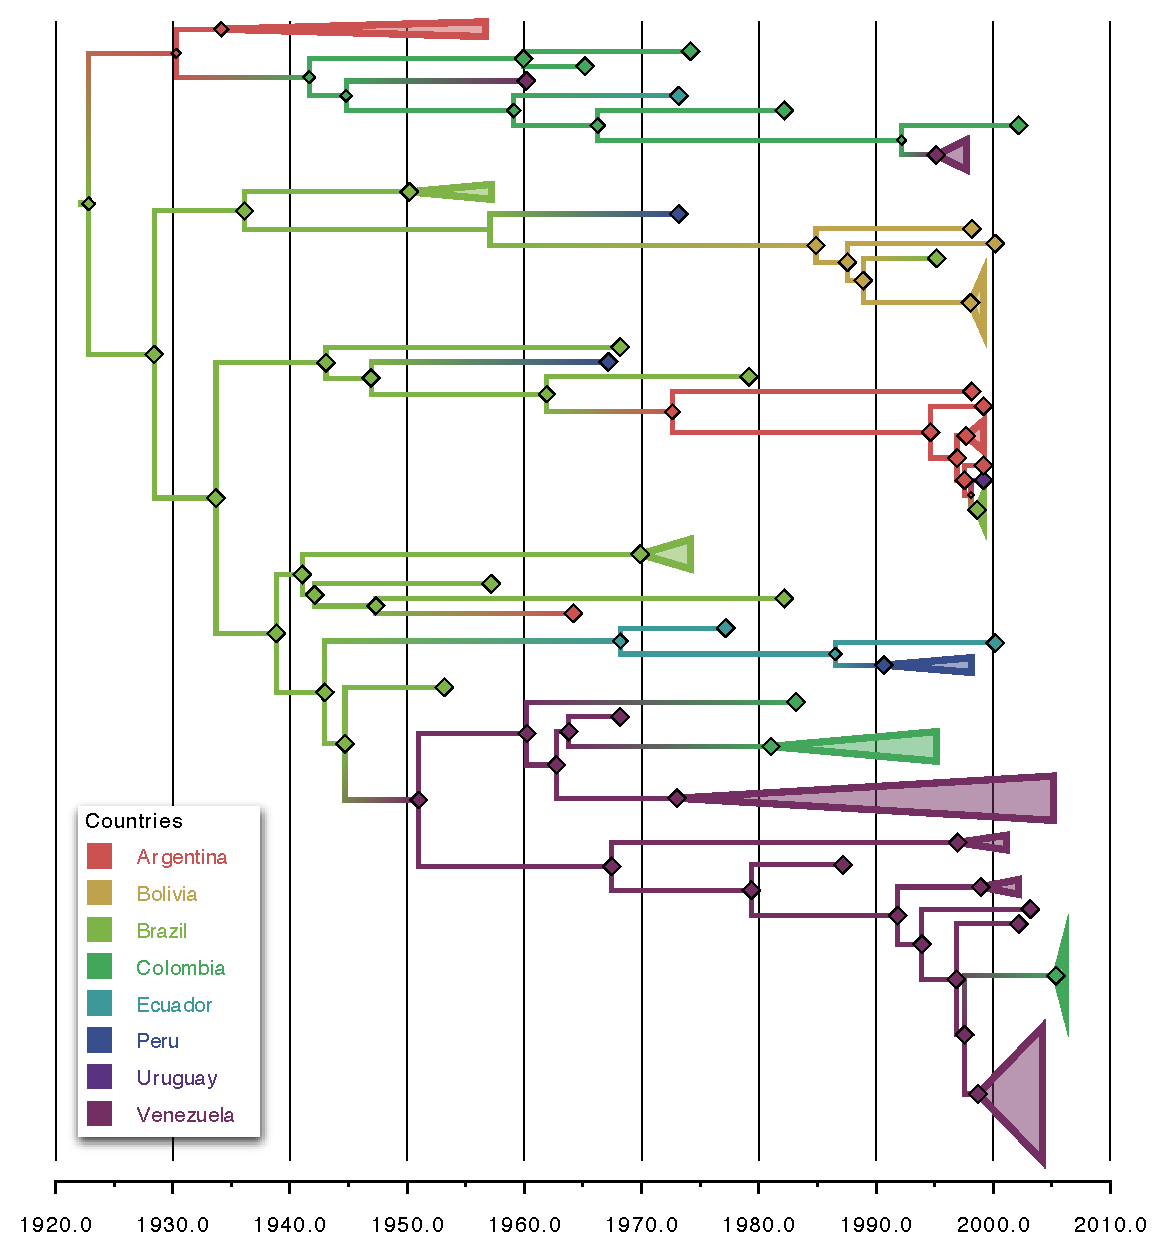
\includegraphics[scale=.45]{FIGURES/A.pdf}}\\
\subfigure[O]{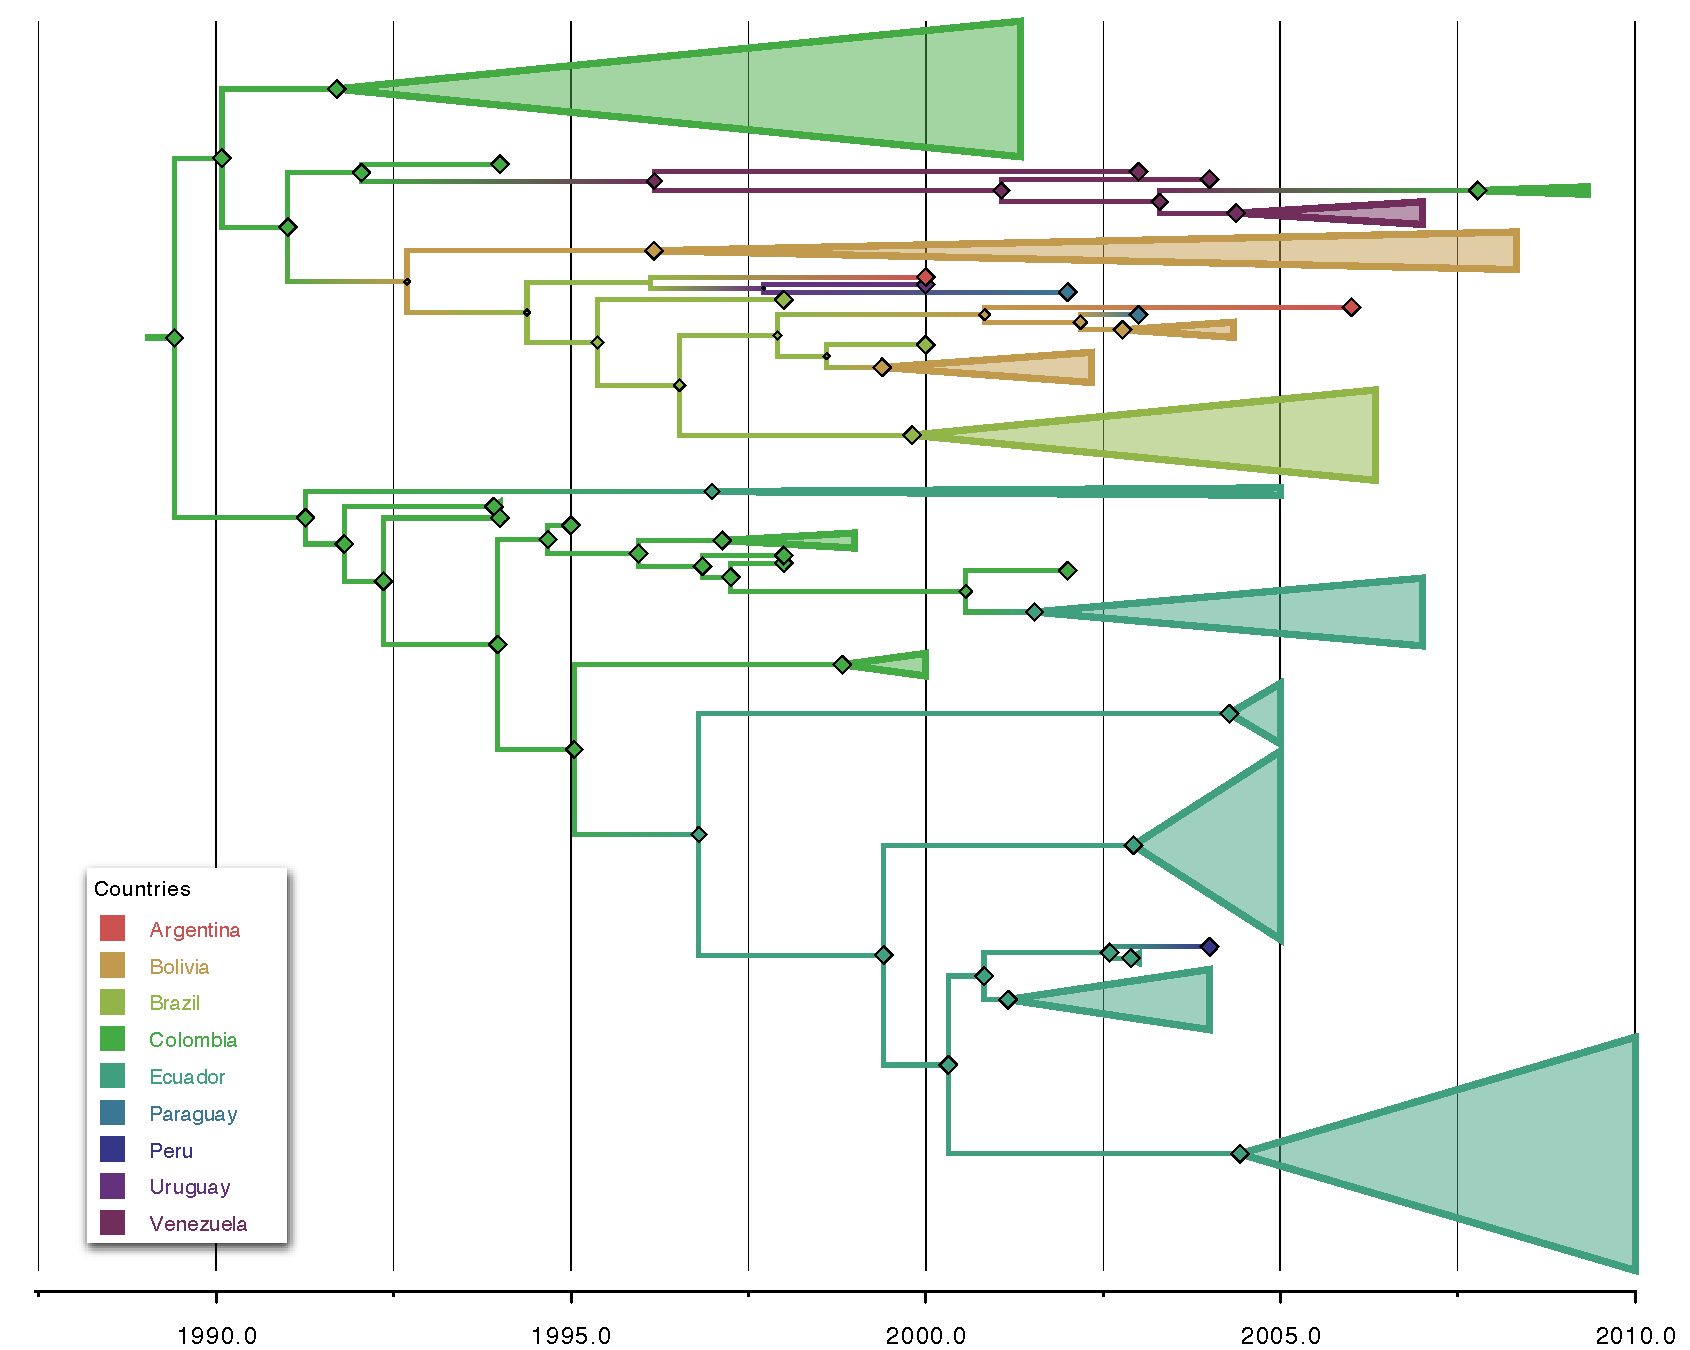
\includegraphics[scale=.30]{FIGURES/O.pdf}}
\end{center}
\caption{}
\label{fig:trees}
\end{figure}
%%%%%%%%%%%%%%%%%%%%%%%%%%
%%%%%%%%%%%%%%%%%%%%%%%%%%
\newpage
\begin{figure}[H]
\begin{center}
\subfigure[A --1945 ]{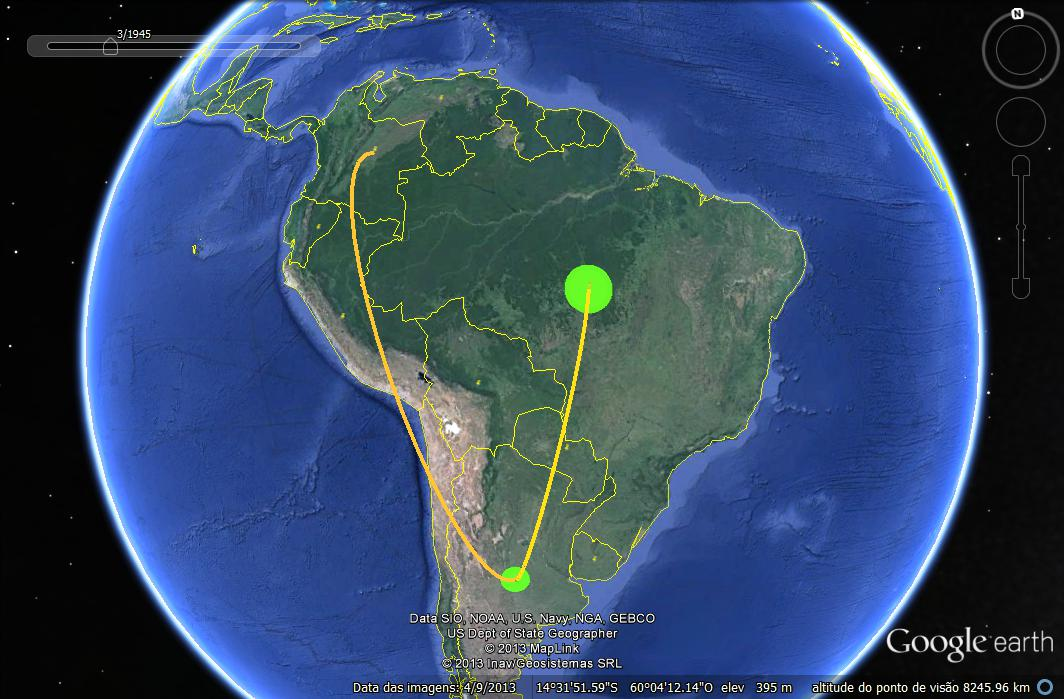
\includegraphics[scale=.20]{FIGURES/A_1945.jpg}}
\subfigure[O --1995 ]{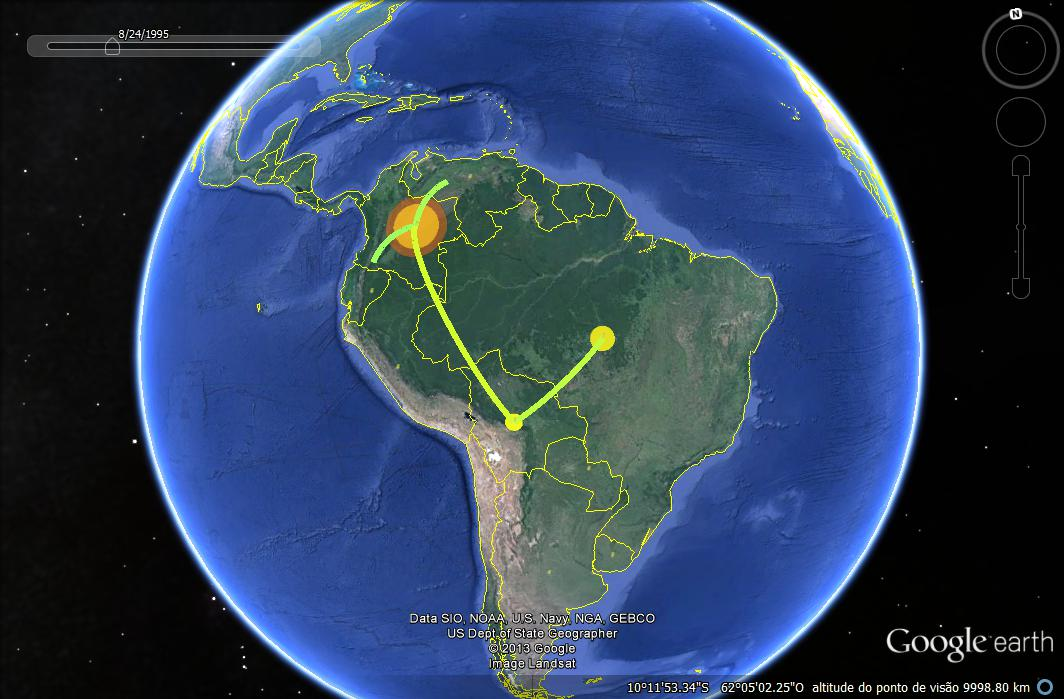
\includegraphics[scale=.20]{FIGURES/O_1995.jpg}}\\
\subfigure[A --1965 ]{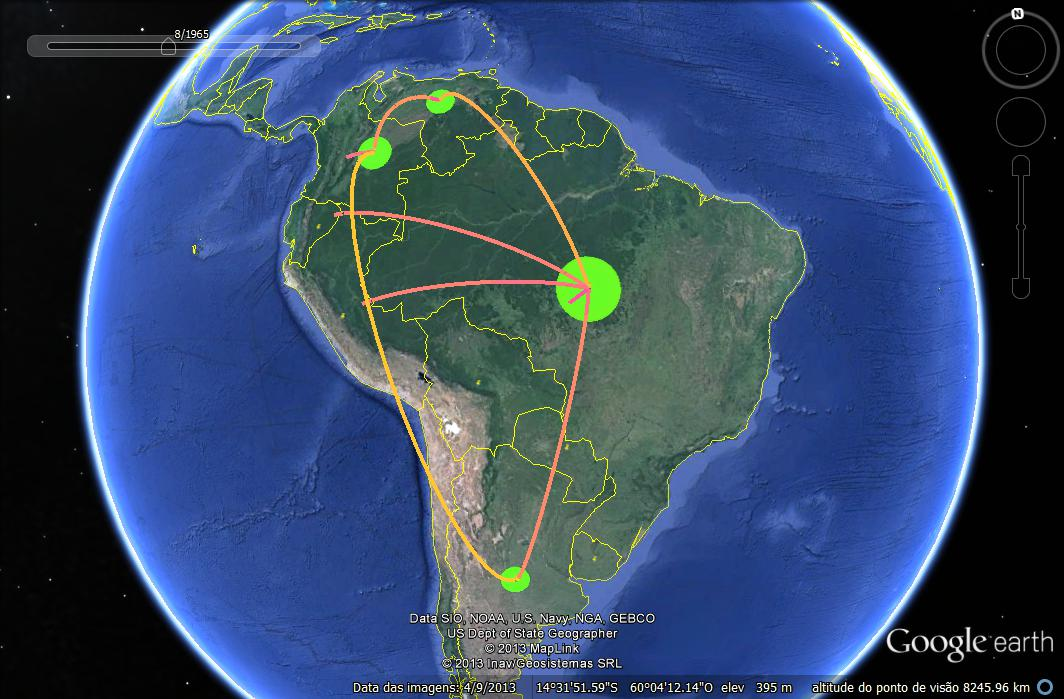
\includegraphics[scale=.20]{FIGURES/A_1965.jpg}}
\subfigure[O --2000 ]{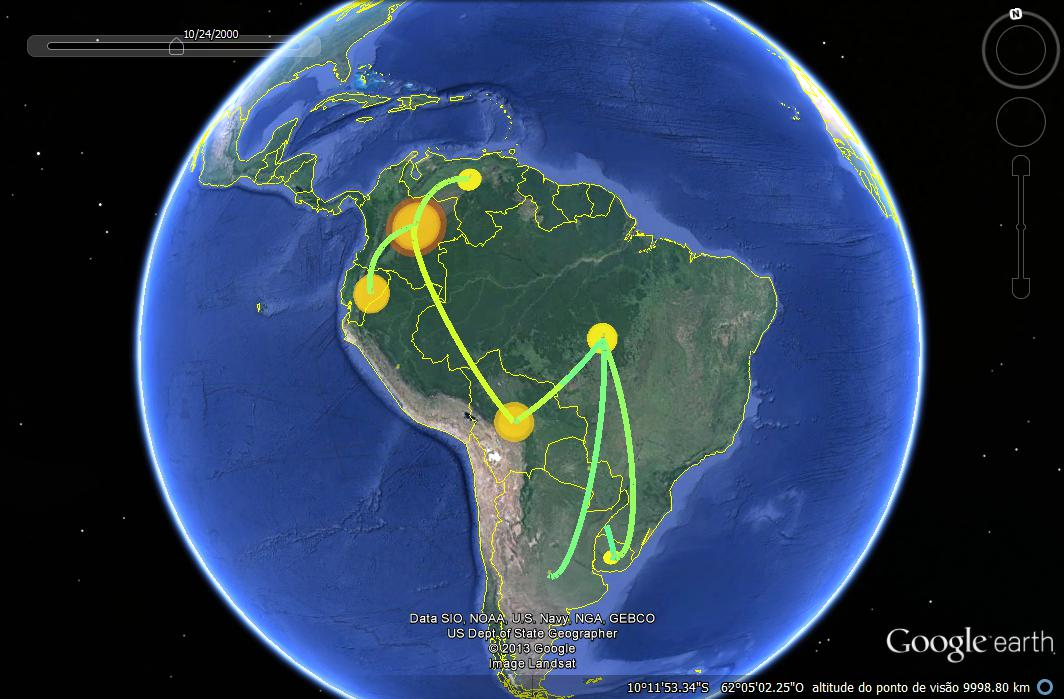
\includegraphics[scale=.20]{FIGURES/O_2000.jpg}}\\
\subfigure[A --1980 ]{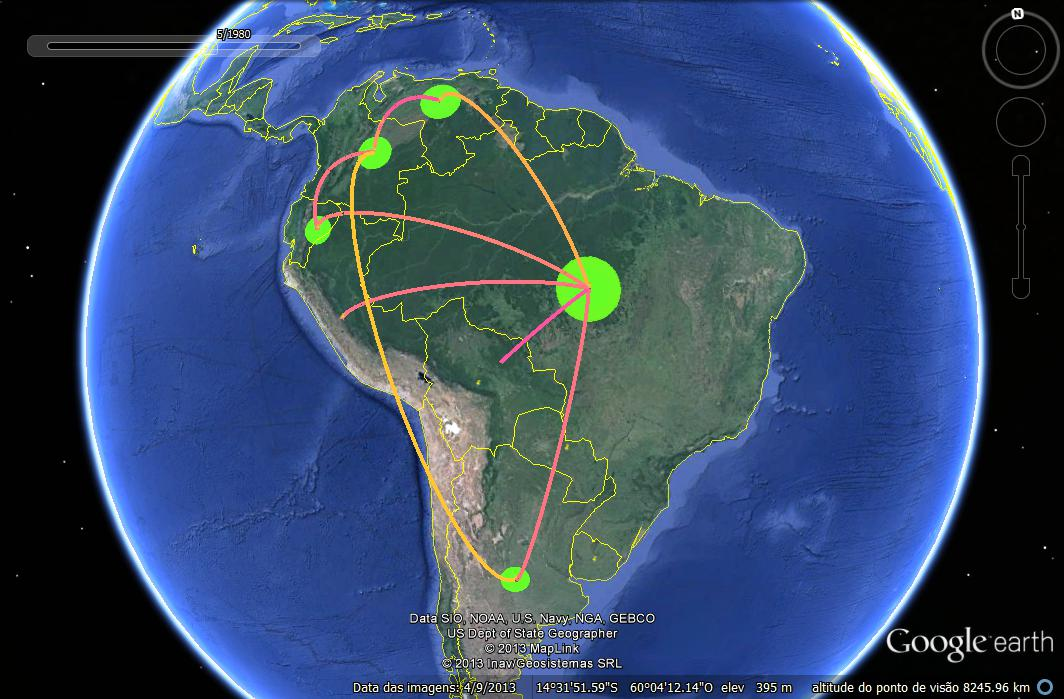
\includegraphics[scale=.20]{FIGURES/A_1980.jpg}}
\subfigure[O --2005 ]{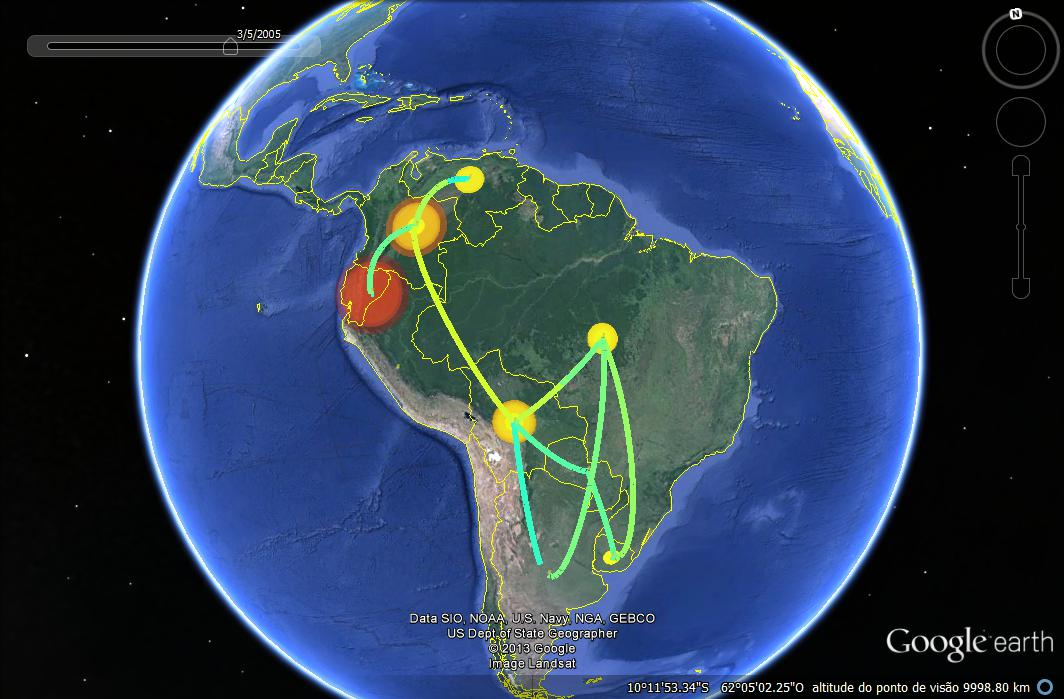
\includegraphics[scale=.20]{FIGURES/O_2005.jpg}}\\
\subfigure[A --2008 ]{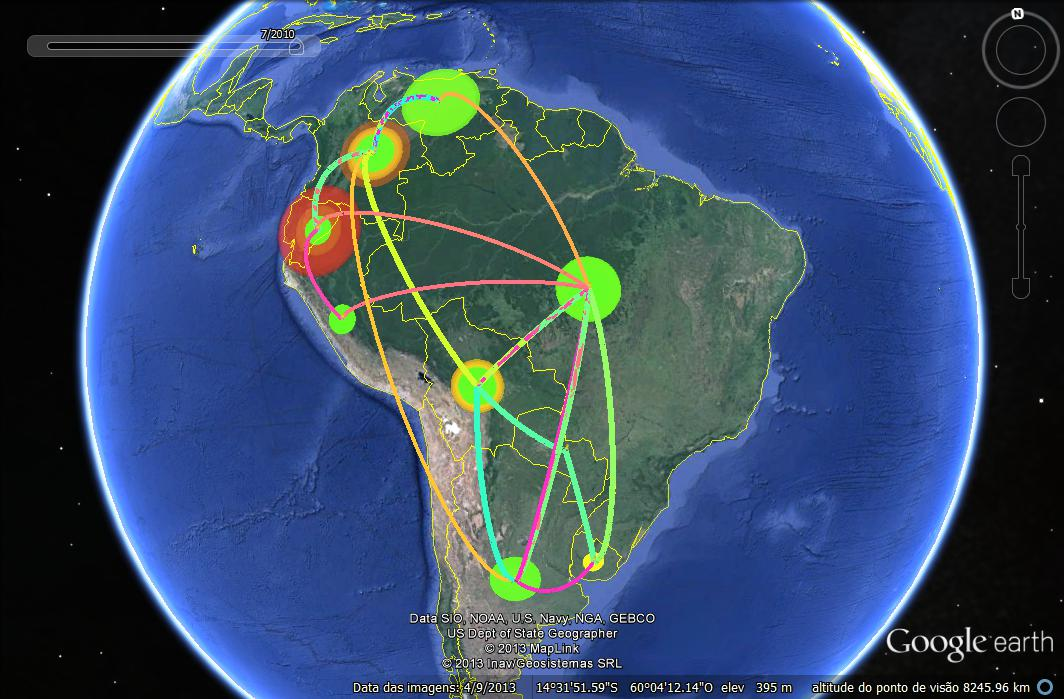
\includegraphics[scale=.20]{FIGURES/A_2008.jpg}}
\subfigure[O --2010 ]{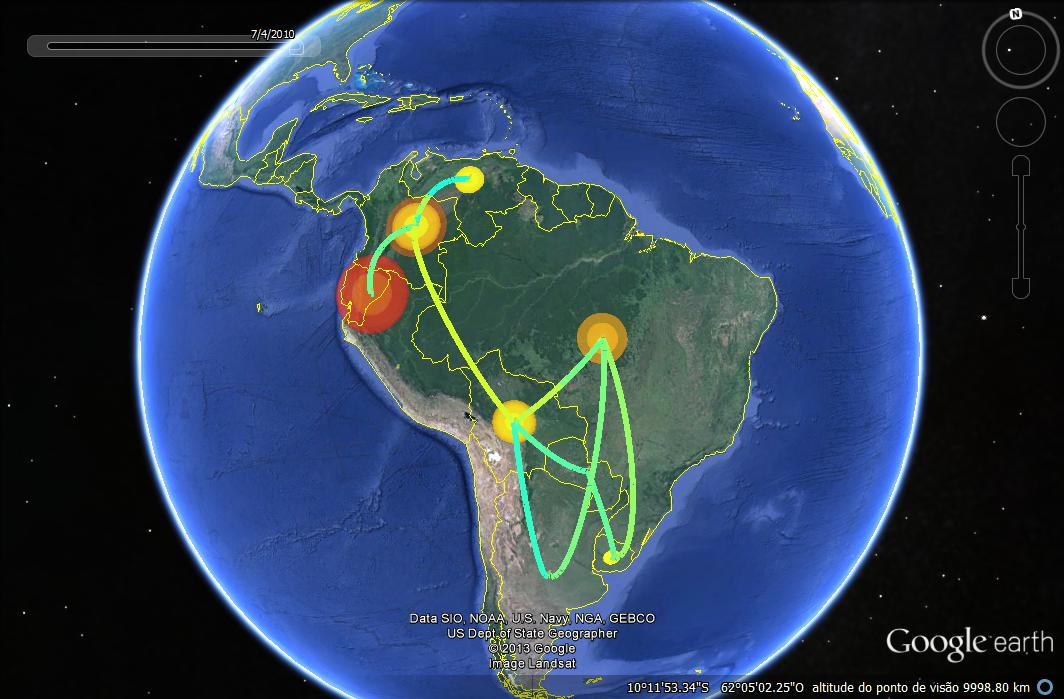
\includegraphics[scale=.20]{FIGURES/O_2010.jpg}}
\end{center}
\caption{}
\label{fig:migration}
\end{figure}
%%%%%%%%%%%%%%%%%%%%%%%%%%
%%%%%%%%%%%%%%%%%%%%%%%%%%
\newpage
\begin{figure}[H]
\begin{center}
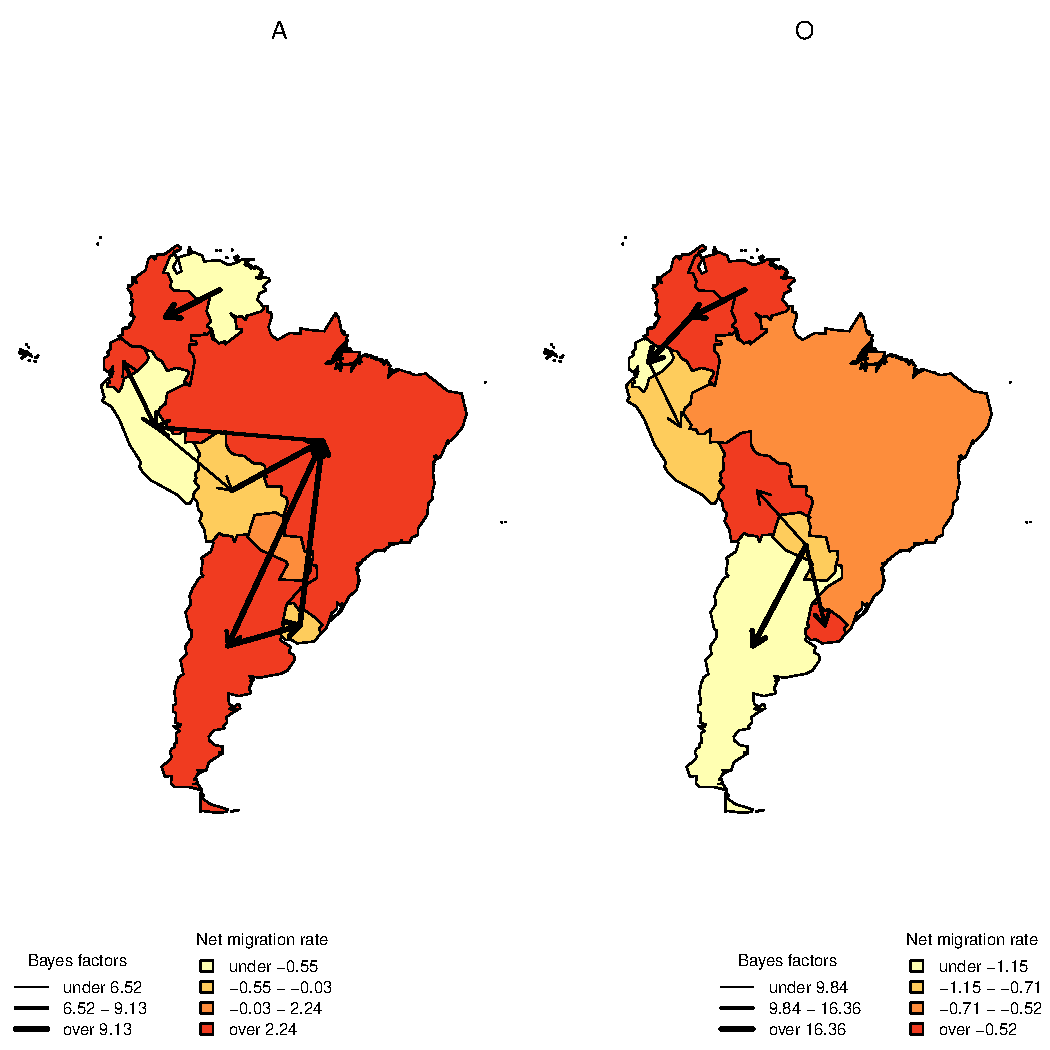
\includegraphics[scale=.90]{FIGURES/MJandBFs.pdf}
\end{center}
\caption{}
\label{fig:mj&BFs}
\end{figure}
%%%%%%%%%%%%%%%%%%%%%%%%%%
%%%%%%%%%%%%%%%%%%%%%%%%%%
\newpage
\begin{figure}[H]
\begin{center}
\subfigure[][]{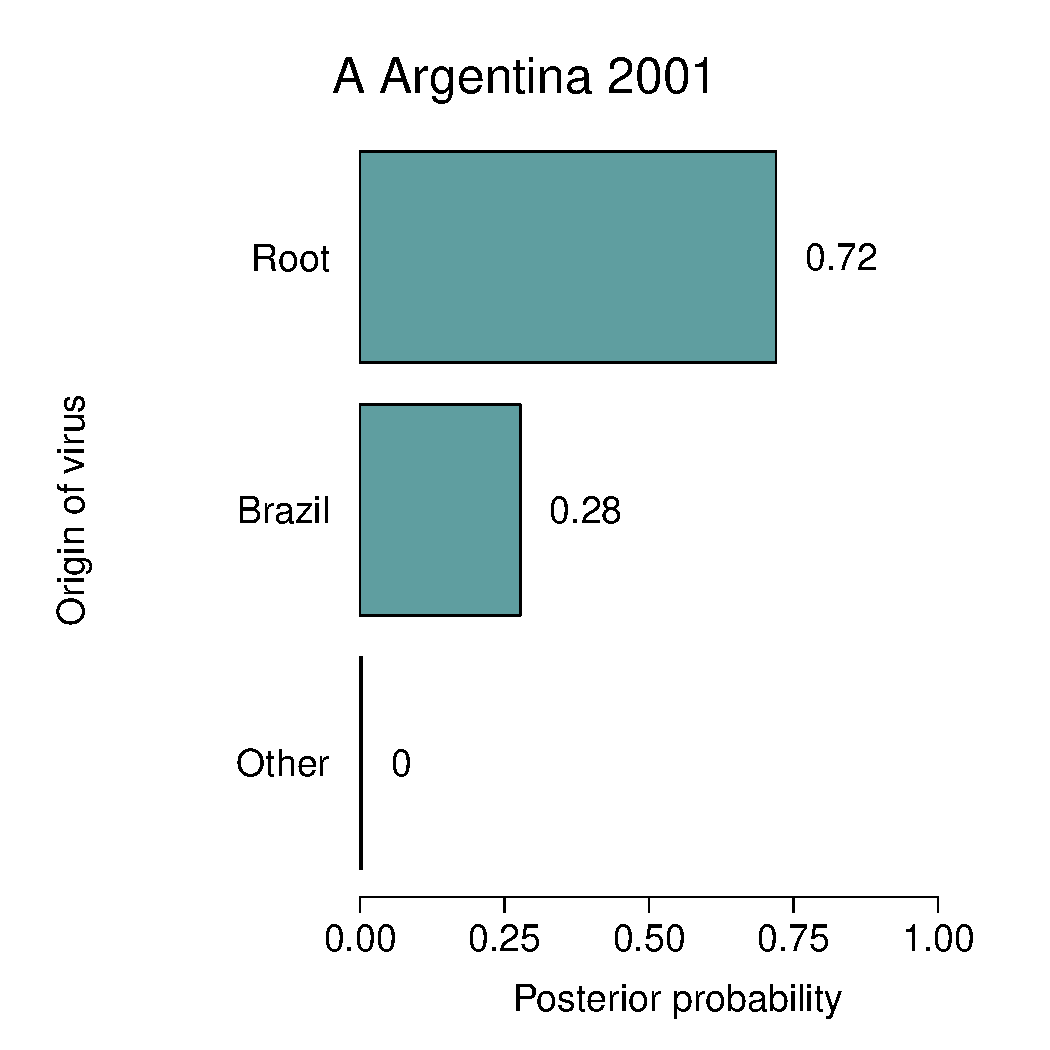
\includegraphics[scale=.40]{FIGURES/Origins_A_Argentina_2001.pdf}}
\subfigure[][]{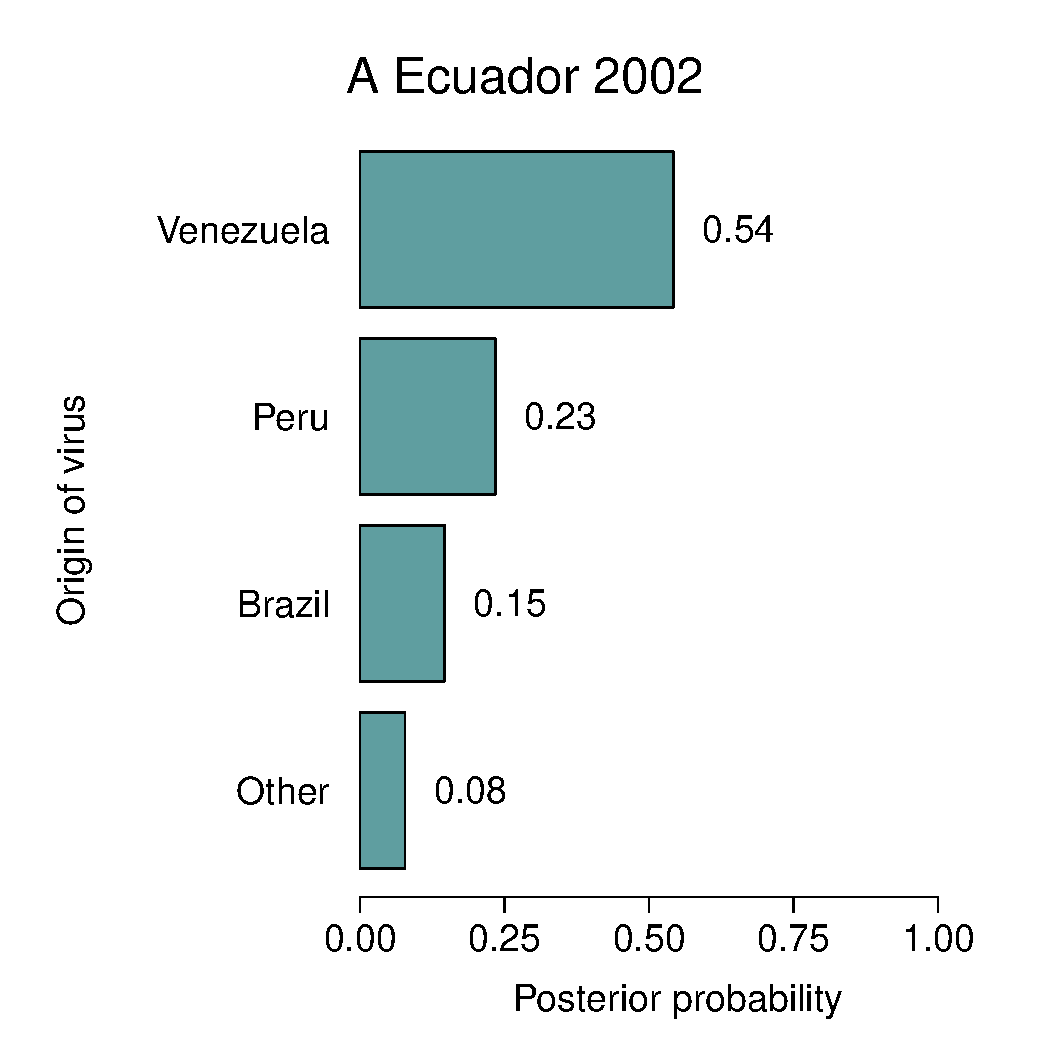
\includegraphics[scale=.40]{FIGURES/Origins_A_Ecuador_2002.pdf}}\\
\subfigure[][]{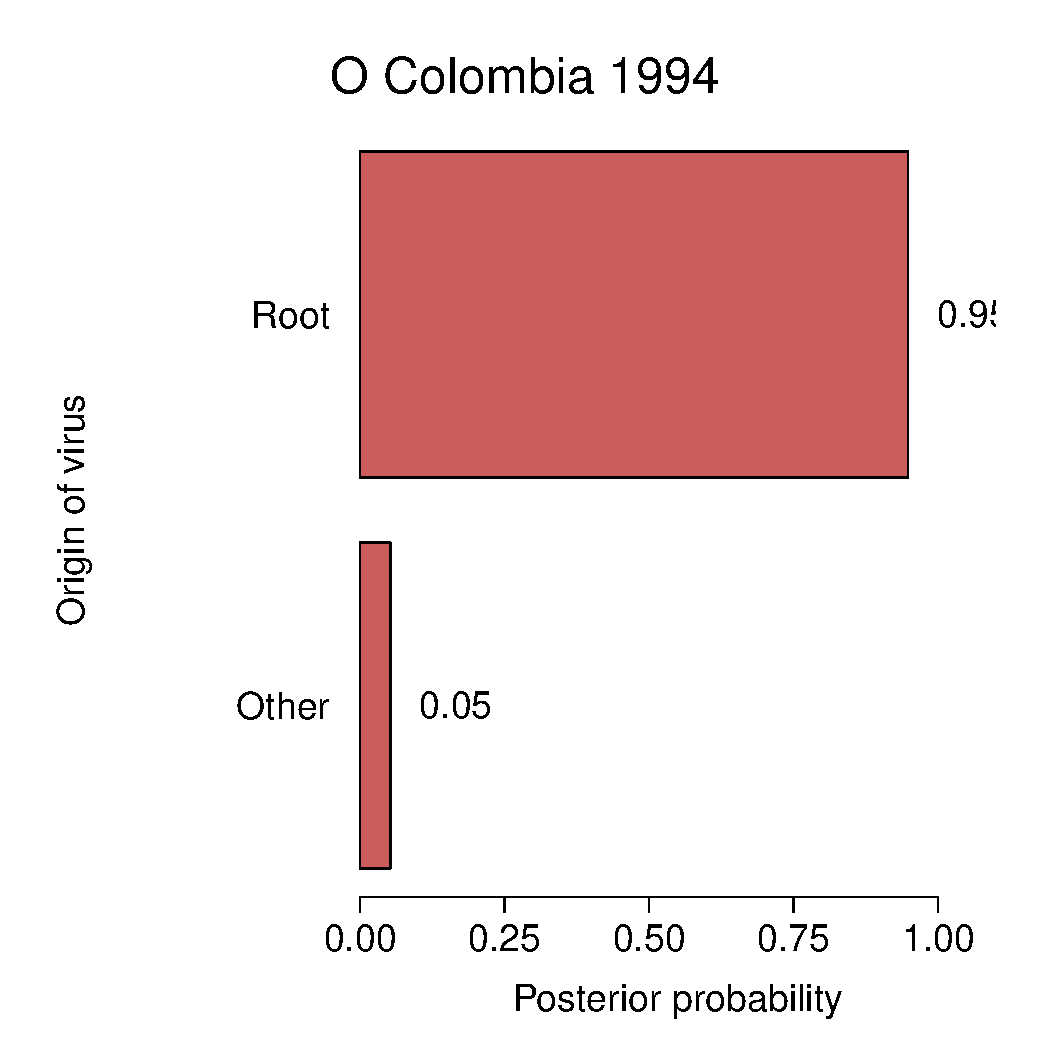
\includegraphics[scale=.40]{FIGURES/Origins_O_Colombia_1994.pdf}}
\subfigure[][]{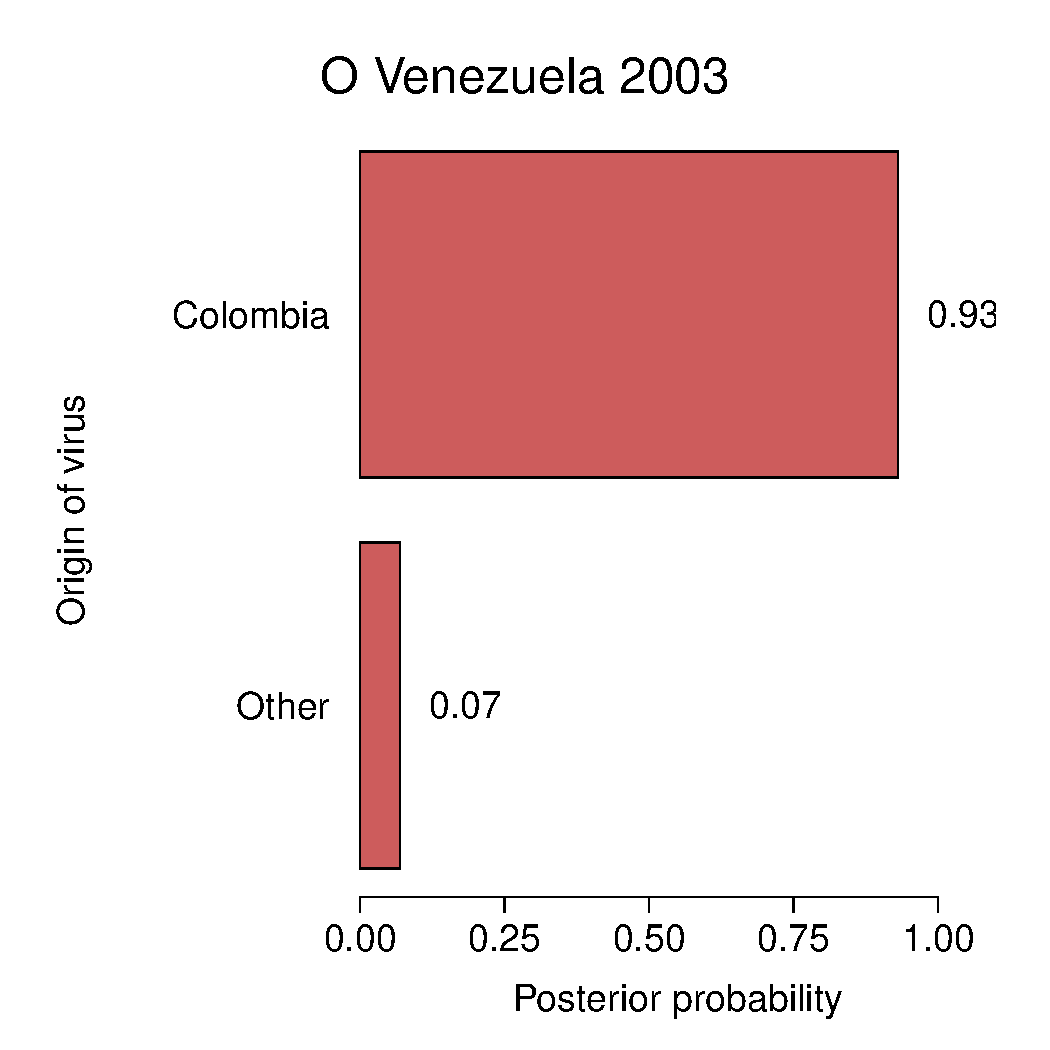
\includegraphics[scale=.40]{FIGURES/Origins_O_Venezuela_2003.pdf}}
\end{center}
\caption{}
\label{fig:epidemictracing}
\end{figure}
%%%%%%%%%%%%%%%%%%%%%%%%%%
%%%%%%%%%%%%%%%%%%%%%%%%%%
\newpage
\begin{figure}[H]
\begin{center}
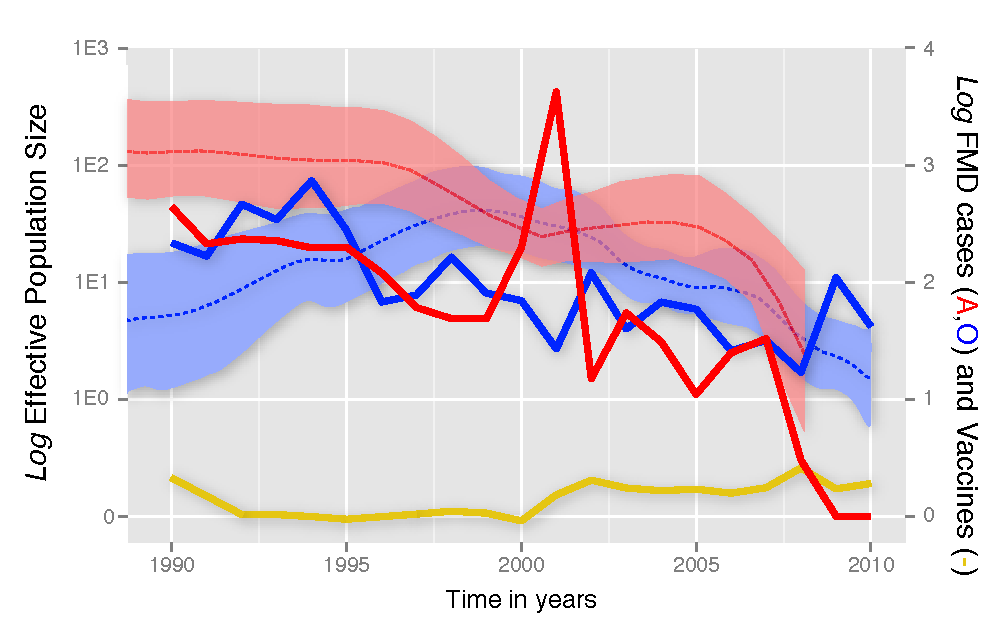
\includegraphics[scale=1.0]{FIGURES/skyride.pdf}
\end{center}
\caption{}
\label{fig:skyride}
\end{figure}
%%%%%%%%%%%%%%%%%%%%%%%%%%
%%%%%%%%%%%%%%%%%%%%%%%%%% 
\newpage
\begin{table}[H]
\caption{
\textbf{Spatial model selection results for epidemiological predictors.}
We assessed the significance of livestock trade in FMDV spread in South America using two marginal likelihood calculation methods, path sampling (PS) and stepping-stone sampling (SS), to estimate (log) marginal likelihoods for each predictor using $64$ path steps and $2$ million iterations per path step, and corresponding Bayes factor (BF) comparisons.
We also present the (log) marginal likelihood estimates for two location priors under which the location rates are estimated, rather than being fixed (as for the livestock predictors).
The results from the equal-rates gamma prior should not be directly compared to those of the livestock trade predictors.
}
\begin{center}
\begin{tabular}{lrrrrrr}
\toprule
 & \multicolumn{3}{c}{Serotype A}& \multicolumn{3}{c}{Serotype O}\\
 \midrule
Predictor & PS & SS & log BF$^2$ & PS & SS & log BF \\
%\hline
Cattle&-12588.76&-12591.26&-27.70&\textbf{-8308.94}&\textbf{-8311.21}& \textbf{13.49}\\
Distance&\textbf{-12557.69}&\textbf{-12559.73}&\textbf{3.83}&-8313.89&-8315.37&9.33\\
Pigs&-12589.33&-12590.94&-27.38&-8325.39&-8326.63&-1.93\\
Sheep&-12570.67&-12572.56&-9.00&-8326.23&-8330.64&-5.94\\
\\
\hline
Equal rates &-12561.98&-12563.56&--&-8321.49&-8324.70&--\\
\bottomrule
\end{tabular}
\end{center}
\begin{flushleft}
\end{flushleft}
\label{tab:preds}
 \end{table}
%%%%%%%%%%%%%%%%%%%%%%%%
%%%%%%%%%%%%%%%%%%%%%%%%
\newpage
\begin{table}[H]
\caption{
\textbf{Inferred root locations for each predictor for both serotypes.} We present most probable country of origin inferred using each predictor, with associated probabilities inside parentheses. 1-- all rates equal; 2-- Probability of being the root; 3-- Kullback-Leibler Divergence.
}
\begin{center}
\begin{tabular}{lcccc}
\toprule
& \multicolumn{2}{c}{Serotype A}&\multicolumn{2}{c}{Serotype O}\\
Predictor& Origin ($Pr$(root)$^2$)& KL$^3$&Origin ($Pr$(root))& KL\\
\midrule
Distance & Argentina ($0.75$)& $3.86$ & Colombia ($0.96$)& $3.76$\\
Sheep    & Brazil ($0.89$) & $3.52$ & Colombia ($0.99$)& $5.91$\\
Pigs      & Colombia ($0.99$)& $5.98$& Colombia ($0.91$)& $4.73$\\
Equal rates$^1$  & Argentina ($0.84$)& $3.78$ &Colombia  ($0.96$)& $3.20$\\
Cattle   & Peru ($0.93$)& $5.17$ & Colombia ($0.95$)& $3.81$\\
 \bottomrule
\end{tabular}
\end{center}
\begin{flushleft}
\end{flushleft}
\label{tab:roots}
 \end{table}
%%%%%%%%%%%%%%%%%%%%%%%%
\end{document}